% ALIGNN / PINK findings deck - build with xelatex (fontspec needs it).
%
%     cd presentation && ./build_alignn.sh
%
% Companion to CGCNN_presentation.tex. That deck explains CGCNN and the
% original reproduction; this one explains ALIGNN's graph construction, then
% presents everything found since - including the results that corrected the
% project's own record. Reuses theme.tex and metrics.tex unchanged.
\documentclass[aspectratio=169]{beamer}
% Custom beamer theme for the CGCNN presentation.
% ================================================
%
% Kept separate from the content file so the visual system - colours, fonts,
% the card/eyebrow building blocks - can be read and adjusted in one place
% without wading through forty frames of prose.
%
% DESIGN
% ------
% Georgia for headings (a serif with the same weight/character as the
% Cambria used in the project's other teaching decks), Avenir Next for body
% text (same role as their Calibri). Both are macOS system fonts, loaded via
% fontspec, so this MUST be built with xelatex or lualatex - not pdflatex.
%
% Cards are TikZ nodes with `text width` set and NO fixed height. That one
% choice eliminates an entire class of bug: a fixed-height text box that
% silently overflows its frame is exactly what an earlier (PowerPoint)
% version of this deck kept getting wrong. A TikZ node sized only by its
% content cannot overflow itself - it grows to fit, by construction.

\usepackage{fontspec}
\setmainfont{Avenir Next}
\setsansfont{Avenir Next}
\newfontfamily\headingfont{Georgia}
\newfontfamily\monofont{Menlo}

\usepackage{tikz}
\usetikzlibrary{arrows.meta,positioning,shapes.geometric,calc,backgrounds,fit}
\usepackage{amsmath,amssymb}
\usepackage{graphicx}
\usepackage{booktabs}
% Both results/ subdirectories are searched in order - every existing
% 
\includegraphics{parity_K_VRH_ens} etc. call (bare filename, no path
% prefix) keeps resolving with no per-call edits after the cgcnn/alignn split.
\graphicspath{{figures/}{../results/cgcnn/}{../results/alignn/}}

% --- Palette ----------------------------------------------------------------
\definecolor{Navy}{HTML}{0F1B33}
\definecolor{SlideBlue}{HTML}{1450AA}
\definecolor{LightBlue}{HTML}{6FA8FF}
\definecolor{SlideGreen}{HTML}{1E8E5A}
\definecolor{SlideAmber}{HTML}{D97B12}
\definecolor{SlideRed}{HTML}{B02A2A}
\definecolor{SlideInk}{HTML}{1F2937}
\definecolor{Muted}{HTML}{5B6B82}
\definecolor{Subtle}{HTML}{AAB6C8}
\definecolor{CardBg}{HTML}{F4F6FA}
\definecolor{CardRule}{HTML}{D8E0EC}
\definecolor{GreenBg}{HTML}{EFF5EF}
\definecolor{GreenRule}{HTML}{C8E0C8}
\definecolor{AmberBg}{HTML}{FDF4E8}
\definecolor{AmberRule}{HTML}{F0D8B8}
\definecolor{BlueBg}{HTML}{E8EFFA}
\definecolor{RedBg}{HTML}{FDF0F0}
\definecolor{RedRule}{HTML}{F0C8C8}
\definecolor{NaColor}{HTML}{7A3FA0}   % matches figures/nacl_*.png
\definecolor{ClColor}{HTML}{1E8E5A}

% --- Bare beamer plumbing: no default chrome, we draw our own -------------
\setbeamertemplate{navigation symbols}{}
\setbeamertemplate{footline}{%
  \hfill\color{Subtle}\scriptsize\insertframenumber\,/\,\inserttotalframenumber\hspace{4mm}\vspace{2mm}
}
\setbeamercolor{background canvas}{bg=white}
\setbeamersize{text margin left=0.85cm, text margin right=0.85cm}
\setbeamertemplate{itemize item}{\textcolor{SlideBlue}{\raisebox{0.15em}{\rule{5pt}{5pt}}}}
\setbeamertemplate{itemize subitem}{\textcolor{Muted}{--}}
\setlength{\parskip}{0pt}

% frametitle is unused throughout - every content frame builds its own header
% with \SlideHeader, so its template is blanked out rather than left to draw
% something nobody positioned.
\setbeamertemplate{frametitle}{}
\setbeamertemplate{headline}{}

% --- The eyebrow + title header every content slide starts with -----------
\newcommand{\Chapter}[0]{}
\newcommand{\SlideHeader}[2]{%
  \par\noindent{\color{SlideBlue}\bfseries\sffamily\fontsize{10}{12}\selectfont #1}\\[2pt]
  \noindent{\color{SlideInk}\bfseries\headingfont\fontsize{19}{22}\selectfont #2}\\[5pt]%
}

% --- A soft card panel; sizes to its content, never the other way round ----
% #1 width  #2 fill  #3 rule (use `none` for no border)  #4 content
\newcommand{\Card}[4]{%
  \begin{tikzpicture}
    \node[rounded corners=4pt, fill=#2,
          draw=#3, line width=0.7pt,
          text width=#1, inner sep=6pt, align=left,
          minimum height=0pt] {#4};
  \end{tikzpicture}%
}
% A card with a coloured accent bar down the left edge - used for the three-
% way "why" explainer boxes.
\newcommand{\AccentCard}[3]{%
  \begin{tikzpicture}
    \node[rounded corners=4pt, fill=CardBg, draw=CardRule, line width=0.7pt,
          text width=#1, inner sep=6pt, align=left,
          minimum height=0pt] (box) {#3};
    \fill[#2, rounded corners=2pt] (box.north west) rectangle
      ($(box.south west)+(0.09,0)$);
  \end{tikzpicture}%
}

% --- The "so what" strip anchored to the bottom of a frame -----------------
\newcommand{\Takeaway}[1]{%
  \vfill
  \begin{tikzpicture}
    \node[rounded corners=4pt, fill=CardBg, draw=none,
          text width=11.3cm, inner sep=6pt, align=left,
          minimum height=0pt] (box) {\sffamily\bfseries\footnotesize\color{SlideInk} #1};
    \fill[SlideBlue, rounded corners=2pt] (box.north west) rectangle
      ($(box.south west)+(0.08,0)$);
  \end{tikzpicture}%
}

% --- Section-divider frame: full navy, one big line of text ---------------
\newenvironment{dividerframe}{%
  \begingroup
  \setbeamercolor{background canvas}{bg=Navy}
  \begin{frame}[plain]
  \vspace{2.6cm}
}{%
  \end{frame}
  \endgroup
}

% --- Title-slide flow pill (the row of stage names on slide 1) ------------
\newcommand{\FlowPill}[1]{%
  \tikz\node[rounded corners=4pt, fill=Navy!60, draw=LightBlue!40,
             line width=0.5pt, text width=2.1cm, align=center,
             inner sep=7pt, font=\sffamily\bfseries\small\color{white}]
             {#1};%
}

\input{metrics.tex}

\input{metrics.tex}

\title{ALIGNN and the PINK Pipeline}
\author{Aizaz Khalid}
\date{}

\newcommand{\PartSlide}[3]{%
  \begingroup
  \setbeamercolor{background canvas}{bg=Navy}
  \begin{frame}[plain]
  \vspace{1.5cm}
  \begin{center}
  {\color{LightBlue}\bfseries\sffamily\large PART #1}\\[8pt]
  {\color{white}\bfseries\headingfont\fontsize{30}{36}\selectfont #2}\\[10pt]
  {\color{Subtle}\sffamily\normalsize #3}
  \end{center}
  \end{frame}
  \endgroup}

\begin{document}

% =============================================================================
%  TITLE
% =============================================================================
\begingroup
\setbeamercolor{background canvas}{bg=Navy}
\begin{frame}[plain]
\vspace{0.9cm}
\begin{center}
{\color{LightBlue}\bfseries\sffamily\large FINDINGS AND METHOD}\\[6pt]
{\color{white}\bfseries\headingfont\fontsize{32}{38}\selectfont
  ALIGNN and the PINK Pipeline}\\[6pt]
{\color{Subtle}\sffamily\large
  A second architecture, the full 554{,}054-material screen,\\
  and what changed when every claim was checked}\\[16pt]
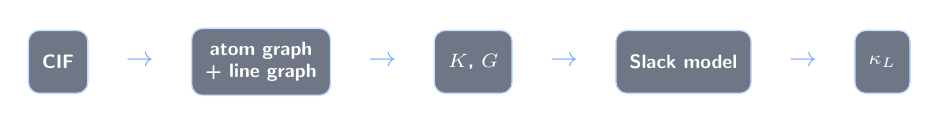
\begin{tikzpicture}[node distance=3.5mm,
  pill/.style={rounded corners=4pt, fill=Navy!60, draw=LightBlue!40,
               line width=0.5pt, minimum height=0.8cm, align=center,
               inner sep=5pt, font=\sffamily\bfseries\scriptsize\color{white}},
  arr/.style={font=\color{LightBlue}\normalsize}]
  \node[pill] (n1) {CIF};
  \node[arr, right=of n1] (a1) {$\rightarrow$};
  \node[pill, right=of a1] (n2) {atom graph\\+ line graph};
  \node[arr, right=of n2] (a2) {$\rightarrow$};
  \node[pill, right=of a2] (n3) {$K$, $G$};
  \node[arr, right=of n3] (a3) {$\rightarrow$};
  \node[pill, right=of a3] (n4) {Slack model};
  \node[arr, right=of n4] (a4) {$\rightarrow$};
  \node[pill, right=of a4] (n5) {$\kappa_L$};
\end{tikzpicture}
\end{center}
\end{frame}
\endgroup

\PartSlide{ONE}{Where the project stands}{PINK reproduced, then extended --- and what the extension is for}

% =============================================================================
\begin{frame}
\SlideHeader{01 \textperiodcentered\ THE PIPELINE}{What PINK does, in one slide}

\begin{columns}[T]
\column{0.54\linewidth}
{\sffamily\footnotesize
PINK (Liu \textit{et al.}, \textit{J. Mater. Inf.} 2025) predicts \textbf{lattice
thermal conductivity} $\kappa_L$ straight from a CIF file, without solving the
phonon Boltzmann transport equation.

\vspace{4pt}
It does that in two stages. A crystal graph network predicts the two elastic
moduli; a closed-form physical model turns those into $\kappa_L$. The physics
stage has no free parameters --- it is the Slack model, not a fit.}

\vspace{5pt}
\Card{6.3cm}{CardBg}{CardRule}{%
  \sffamily\footnotesize
  \textbf{Why this is worth doing}\\[3pt]
  A full DFT + PBTE calculation of $\kappa_L$ takes days per material. This
  takes about a sixth of a second. That is the difference between checking a
  handful of candidates and screening half a million.}

\column{0.42\linewidth}
{\sffamily\footnotesize\color{Muted} The two stages:}\\[4pt]
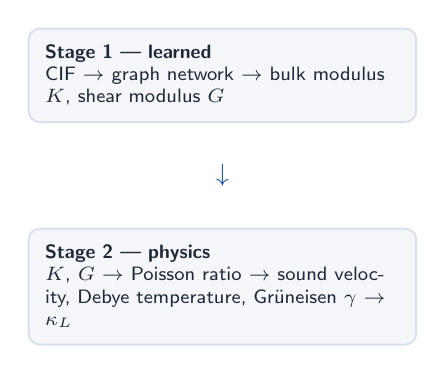
\begin{tikzpicture}[node distance=4mm,
  box/.style={rounded corners=4pt, fill=CardBg, draw=CardRule, line width=0.7pt,
              text width=4.5cm, align=left, inner sep=6pt,
              font=\sffamily\scriptsize\color{SlideInk}},
  arr/.style={font=\color{SlideBlue}\small}]
  \node[box] (b1) {\textbf{Stage 1 --- learned}\\ CIF $\rightarrow$ graph network
                   $\rightarrow$ bulk modulus $K$, shear modulus $G$};
  \node[arr, below=of b1] (a1) {$\downarrow$};
  \node[box, below=of a1] (b2) {\textbf{Stage 2 --- physics}\\ $K$, $G$
                   $\rightarrow$ Poisson ratio $\rightarrow$ sound velocity,
                   Debye temperature, Gr\"uneisen $\gamma$ $\rightarrow$ $\kappa_L$};
\end{tikzpicture}
\end{columns}

\Takeaway{The network never sees a thermal conductivity. It learns elasticity;
the physics does the rest.}
\end{frame}

% =============================================================================

\begin{frame}
\SlideHeader{01b \textperiodcentered\ THE PIPELINE}{The paper's own Figure 1}

\begin{center}
\includegraphics[width=0.83\linewidth]{figures/paper_fig1_workflow.png}
\end{center}

\vspace{-2pt}
{\sffamily\scriptsize
Reproduced from Liu \textit{et al.}, \textit{J.\ Mater.\ Inf.} 2025, 5, 12
(CC BY 4.0). \textbf{Blue} the input CIF; \textbf{yellow} the only learned step;
\textbf{purple and green} the closed-form physics; \textbf{red} the answer. The
boxed equation is the one this project reports --- note $\kappa_L \propto
e^{-\gamma}$, an \emph{exponential} dependence on the Gr\"uneisen parameter.}
\end{frame}

\begin{frame}
\SlideHeader{02 \textperiodcentered\ THE PIPELINE}{What this project added}

\begin{columns}[T]
\column{0.48\linewidth}
\AccentCard{5.6cm}{SlideBlue}{%
  \sffamily\footnotesize
  \textbf{A second architecture}\\[2pt]
  ALIGNN, trained on the identical split, so the two can be compared without
  caveats. It beats the CGCNN ensemble on both moduli.}
\vspace{4pt}
\AccentCard{5.6cm}{SlideGreen}{%
  \sffamily\footnotesize
  \textbf{The full screen, twice}\\[2pt]
  All 33{,}118 GNoME candidates scored by both architectures --- the paper's
  own headline experiment, run independently.}
\vspace{4pt}
\AccentCard{5.6cm}{SlideAmber}{%
  \sffamily\footnotesize
  \textbf{Validation against measurement}\\[2pt]
  45 materials with experimentally measured $\kappa_L$, not model-vs-model.}

\column{0.48\linewidth}
\AccentCard{5.6cm}{Muted}{%
  \sffamily\footnotesize
  \textbf{And --- the part that took longest ---}\\[2pt]
  every headline claim re-checked against the artefacts that produced it.
  Four evaluation failure modes were found, each of which inflates reported
  performance. Three numbers already written down turned out to be wrong.}

\vspace{6pt}
{\sffamily\footnotesize
Parts 6 and 7 of this deck are those checks. They are the least glamorous
material here and probably the most useful to anyone else building the same
kind of screen.}
\end{columns}

\Takeaway{Two architectures agreeing is evidence. Two architectures agreeing
because they share a mistake is not --- so most of the work went into telling
those apart.}
\end{frame}

\PartSlide{TWO}{ALIGNN: from CIF to two graphs}{The one structural idea that separates it from CGCNN}

% =============================================================================
\begin{frame}
\SlideHeader{03 \textperiodcentered\ CIF TO GRAPH}{Why a second architecture at all}

{\sffamily\footnotesize
A single model that scores well can be right for the wrong reason. Two models
that share only the training data and the physics --- not the architecture ---
give an independent check: where they agree, the signal is unlikely to be an
artefact of either one.

\vspace{4pt}
ALIGNN was chosen because its difference from CGCNN is \textbf{physically
motivated rather than incidental}. It is not a bigger CGCNN or a differently
tuned one. It sees something CGCNN structurally cannot: \textbf{bond angles}.}

\vspace{6pt}
\begin{columns}[T]
\column{0.47\linewidth}
\Card{5.6cm}{CardBg}{CardRule}{%
  \sffamily\footnotesize
  \textbf{What CGCNN encodes}\\[3pt]
  Which atoms exist, which are bonded, and \emph{how far apart} they are.
  A pure two-body description.}
\column{0.47\linewidth}
\Card{5.6cm}{CardBg}{CardRule}{%
  \sffamily\footnotesize
  \textbf{What ALIGNN adds}\\[3pt]
  The \emph{angles} between bonds --- a three-body term. Elastic response to
  shear depends on how bonds resist \emph{bending}, not only stretching.}
\end{columns}

\Takeaway{Shear modulus is a bond-bending property. A model blind to angles is
being asked to infer it indirectly.}
\end{frame}

% =============================================================================
\begin{frame}
\SlideHeader{04 \textperiodcentered\ CIF TO GRAPH}{Step 1 --- the CIF, and finding neighbours}

\begin{columns}[T]
\column{0.50\linewidth}
{\sffamily\footnotesize
Identical to CGCNN's start: a CIF gives lattice vectors, fractional coordinates
and the element at each site. Neighbours come from a \textbf{periodic distance
search}, so an atom near a face still finds those across the boundary.}

\vspace{5pt}
\Card{6.0cm}{CardBg}{CardRule}{%
  \sffamily\footnotesize
  \textbf{The two settings that define the graph}\\[3pt]
  \texttt{cutoff = 5.0} \AA\ --- the radius within which a neighbour counts\\[2pt]
  \texttt{max\_neighbors = 12} --- the cap per atom\\[3pt]
  {\color{Muted}Read from the trained model's own config --- building 8.0 \AA\
  graphs for a 5.0 \AA\ model would feed it an unseen neighbourhood.}}

\column{0.46\linewidth}
{\sffamily\footnotesize\color{Muted} What comes out of this step:}\\[3pt]
\begin{tabular}{@{}ll@{}}
\toprule
\footnotesize quantity & \footnotesize becomes \\
\midrule
\footnotesize element at site $i$ & \footnotesize node feature $\mathbf{v}_i$ \\
\footnotesize bond $i \rightarrow j$ & \footnotesize edge $e_{ij}$ \\
\footnotesize distance $r_{ij}$ & \footnotesize edge feature \\
\footnotesize angle $\theta_{jik}$ & \footnotesize \textbf{ALIGNN only} \\
\bottomrule
\end{tabular}

\vspace{6pt}
{\sffamily\footnotesize
Node features come from the same 92-dimensional element table CGCNN uses
(\texttt{atom\_features = cgcnn} in the config), so the two architectures start
from identical chemistry.}
\end{columns}
\end{frame}

% =============================================================================
\begin{frame}
\SlideHeader{05 \textperiodcentered\ CIF TO GRAPH}{Step 2 --- one crystal becomes \emph{two} graphs}

\begin{center}
\includegraphics[width=0.97\linewidth]{figures/alignn_line_graph.png}
\end{center}

\vspace{-2pt}
{\sffamily\footnotesize
\textbf{A} the real motif: a centre atom, its neighbours, and the angles between
the bonds. \quad
\textbf{B} the \textbf{atom graph} $\mathcal{G}$ --- atoms are nodes, bonds are
edges. This is exactly what CGCNN builds, and where CGCNN stops. \quad
\textbf{C} the \textbf{line graph} $\mathcal{L}$ --- every \emph{bond} of
$\mathcal{G}$ becomes a \emph{node}, and two bonds sharing an atom are joined by
an edge that carries the angle between them.}

\Takeaway{The line graph is a graph \emph{of the bonds}. Its edges are angles ---
which is how a message-passing network gets access to three-body geometry.}
\end{frame}

% =============================================================================

\begin{frame}
\SlideHeader{05b \textperiodcentered\ CIF TO GRAPH}{The same thing on a real file: NaCl}

\begin{center}
\includegraphics[width=0.97\linewidth]{figures/nacl_alignn_graphs.png}
\end{center}

\vspace{-2pt}
{\sffamily\scriptsize
Computed from \texttt{nacl.cif} at \textbf{ALIGNN's own} settings --- cutoff
5.0 \AA, max 12 neighbours, read from the trained model's config. \textbf{8
atoms, 96 bond edges, 528 angle edges:} each atom keeps 12 neighbours and so
contributes $\binom{12}{2} = 66$ angles. \textbf{The line graph carries
5.5$\times$ more edges than the atom graph} --- that is what seeing angles
costs.}
\end{frame}

\begin{frame}
\SlideHeader{06 \textperiodcentered\ CIF TO GRAPH}{Why the line graph is the right construction}

\begin{columns}[T]
\column{0.50\linewidth}
{\sffamily\footnotesize
A message-passing network updates a node from its neighbours. On the atom graph
alone, the only geometric quantity available to a message is the bond
\emph{length} $r_{ij}$ --- there is nowhere for an angle to live, because an
angle is a property of a \emph{pair} of bonds, not of one.

\vspace{4pt}
Promoting bonds to nodes solves that exactly. In $\mathcal{L}$, a pair of bonds
is an \emph{edge}, and an edge is precisely where a feature can be attached.}

\vspace{5pt}
\Card{6.0cm}{CardBg}{CardRule}{%
  \sffamily\footnotesize
  \textbf{Counting the geometry}\\[3pt]
  An atom with $n$ neighbours contributes $n$ nodes to $\mathcal{L}$ and
  $\binom{n}{2}$ angle edges. At \texttt{max\_neighbors = 12} that is up to
  66 angles per atom --- the reason ALIGNN costs more per structure than
  CGCNN does.}

\column{0.46\linewidth}
{\sffamily\footnotesize\color{Muted} Angle encoding:}\\[3pt]
{\sffamily\footnotesize
The angle is fed as $\cos\theta_{jik}$ expanded on a radial basis, the same way
distances are. Using the cosine rather than the angle keeps the feature smooth
where it matters and avoids a discontinuity at $0$ and $\pi$.}

\vspace{6pt}
\Card{5.4cm}{CardBg}{CardRule}{%
  \sffamily\footnotesize
  \textbf{A sanity check}\\[3pt]
  A cubic cell and a sheared one with identical bond lengths are
  \emph{indistinguishable} to a two-body descriptor, and distinct to ALIGNN.}
\end{columns}
\end{frame}

% =============================================================================
\begin{frame}
\SlideHeader{07 \textperiodcentered\ CIF TO GRAPH}{Step 3 --- the ALIGNN layer alternates between them}

\begin{columns}[T]
\column{0.52\linewidth}
{\sffamily\footnotesize
One ALIGNN layer is two coupled updates, run in order:}

\vspace{5pt}
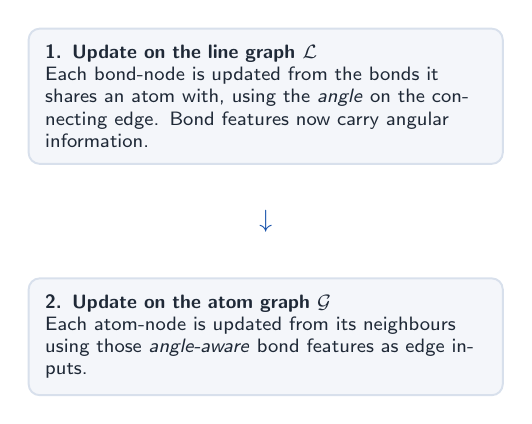
\begin{tikzpicture}[node distance=4.5mm,
  box/.style={rounded corners=4pt, fill=CardBg, draw=CardRule, line width=0.7pt,
              text width=5.6cm, align=left, inner sep=6pt,
              font=\sffamily\scriptsize\color{SlideInk}},
  arr/.style={font=\color{SlideBlue}\small}]
  \node[box] (b1) {\textbf{1. Update on the line graph $\mathcal{L}$}\\
    Each bond-node is updated from the bonds it shares an atom with, using the
    \emph{angle} on the connecting edge. Bond features now carry angular
    information.};
  \node[arr, below=of b1] (a1) {$\downarrow$};
  \node[box, below=of a1] (b2) {\textbf{2. Update on the atom graph $\mathcal{G}$}\\
    Each atom-node is updated from its neighbours using those
    \emph{angle-aware} bond features as edge inputs.};
\end{tikzpicture}



\column{0.44\linewidth}
\Card{5.4cm}{CardBg}{CardRule}{%
  \sffamily\footnotesize
  \textbf{Then, identically to CGCNN}\\[3pt]
  Pool the atom-node vectors over the cell (mean), pass through a small
  fully-connected head, and emit one number.\\[3pt]
  Trained on $\log_{10}$ of the modulus, so the loss is relative --- a 10 GPa
  error on a 20 GPa crystal is penalised far more than on a 300 GPa one.}

\vspace{4pt}
{\sffamily\scriptsize\color{Muted}
Two separate models, one per target --- as in the CGCNN arm.}
\end{columns}
\end{frame}

% =============================================================================
\begin{frame}
\SlideHeader{08 \textperiodcentered\ CIF TO GRAPH}{CGCNN and ALIGNN, side by side}

\begin{center}
\begin{tabular}{@{}lll@{}}
\toprule
& \textbf{CGCNN} & \textbf{ALIGNN} \\
\midrule
graphs built        & atom graph only            & atom graph \textbf{+ line graph} \\
geometry seen       & bond lengths (two-body)    & lengths \textbf{+ angles} (three-body) \\
node features       & 92-dim element table       & same 92-dim table \\
neighbour rule      & cutoff + max-neighbour cap & same (5.0 \AA, 12) \\
message passing     & on $\mathcal{G}$           & alternating $\mathcal{L}$ then $\mathcal{G}$ \\
cost per structure  & lower                      & higher (up to $\binom{12}{2}$ angles/atom) \\
\midrule
models trained        & 3 per target (ensembled)   & \textbf{1 per target} \\
uncertainty estimate  & ensemble spread            & \textbf{none} \\
bulk $K$ MAE $\log_{10}$   & \KOneMae\ one / \KEnsMae\ ens. & \textbf{0.0539} \\
shear $G$ MAE $\log_{10}$  & \GOneMae\ one / \GEnsMae\ ens. & \textbf{0.0725} \\
\bottomrule
\end{tabular}
\end{center}

\vspace{4pt}
{\sffamily\footnotesize
Same 10{,}987 crystals, same \texttt{split\_seed = 42}, same 1{,}648 held-out
test set, both trained the full 150 epochs with no early stop. The comparison is
architecture and nothing else.}

\Takeaway{A \emph{single} ALIGNN beats a three-model CGCNN ensemble --- 23\%
better on bulk single-vs-single. It is also the only model improvement here that
survived the re-scoring in Part 7. No ALIGNN ensemble has been trained, so it
carries no uncertainty interval and its own best number is untested.}
\end{frame}

\PartSlide{THREE}{Training and accuracy}{The dataset, the fit, and where it fails}

% =============================================================================
\begin{frame}
\SlideHeader{09 \textperiodcentered\ THE DATA}{The training set --- PINK's Figure 4, our version}

\begin{center}
\includegraphics[width=0.74\linewidth]{figures/pink_fig4_dataset_stats.png}
\end{center}

{\sffamily\footnotesize
The matbench elastic benchmark: \textbf{10{,}987 crystals} with DFT-computed
$K_{VRH}$ and $G_{VRH}$, split 70/15/15 at \texttt{split\_seed = 42} into
7{,}691 train / 1{,}648 validation / 1{,}648 test. Both moduli are strongly
right-skewed, which is why everything here is trained on $\log_{10}$.}

\Takeaway{The soft tail in panel B is thin --- and it is exactly the region the
whole screen is aimed at. That imbalance shows up again in Part 3 and Part 7.}
\end{frame}

% =============================================================================
\begin{frame}
\SlideHeader{10 \textperiodcentered\ RESULTS}{Predicted vs DFT --- PINK's Figure 5, CGCNN arm}

\begin{columns}[T]
\column{0.49\linewidth}
\begin{center}
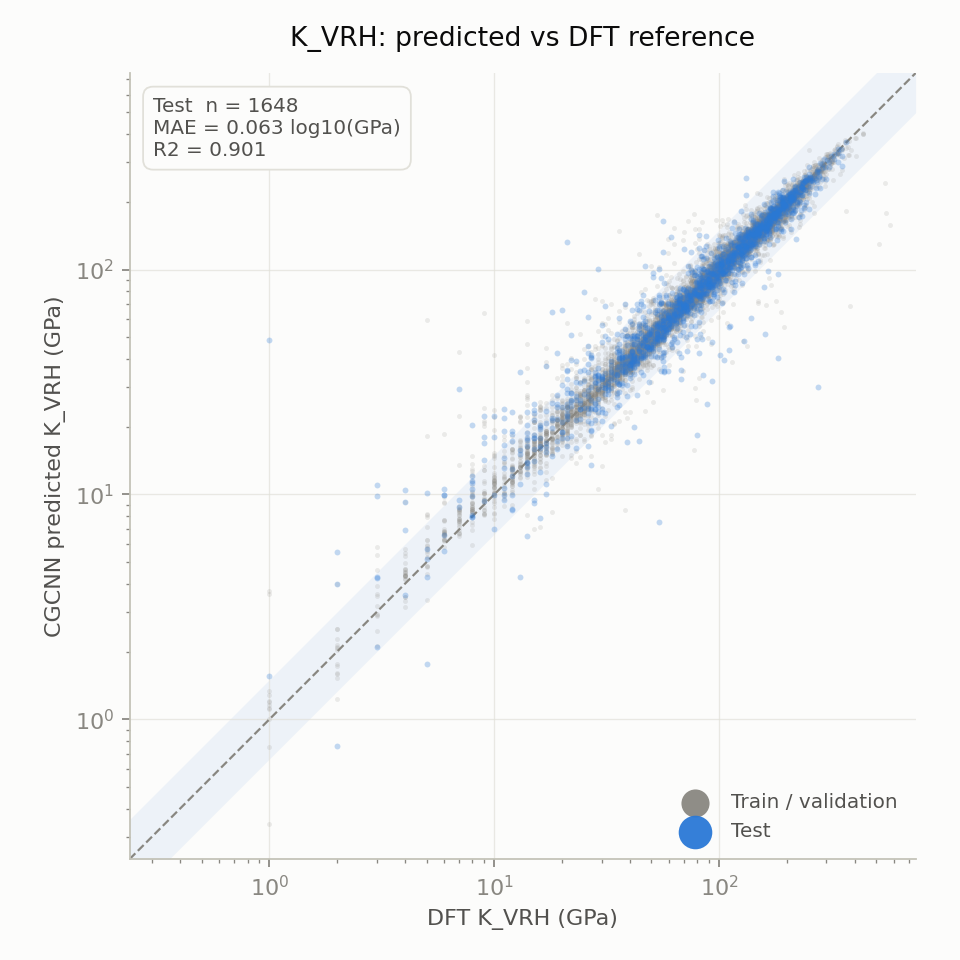
\includegraphics[width=\linewidth]{../results/cgcnn/parity_K_VRH_ens.png}
\end{center}
\column{0.49\linewidth}
\begin{center}
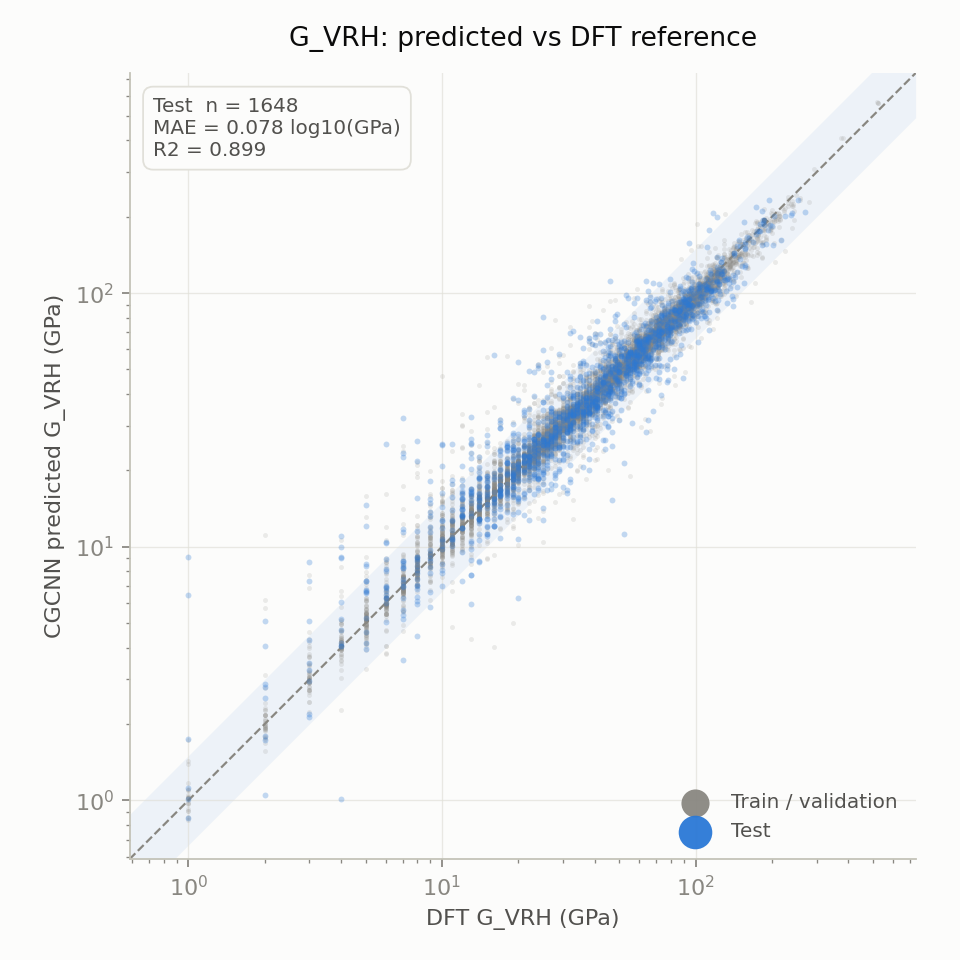
\includegraphics[width=\linewidth]{../results/cgcnn/parity_G_VRH_ens.png}
\end{center}
\end{columns}

\vspace{2pt}
{\sffamily\footnotesize
The 3-model ensemble on the 1{,}648 held-out crystals.
Bulk: MAE $\KEnsMae$ $\log_{10}$, $R^2 = \KEnsRtwo$, \KEnsGpa\ GPa.
Shear: MAE $\GEnsMae$, $R^2 = \GEnsRtwo$, \GEnsGpa\ GPa.
Both beat the paper's own stated ``MAE $<13$'' in raw GPa.}
\end{frame}

% =============================================================================
\begin{frame}
\SlideHeader{11 \textperiodcentered\ RESULTS}{Predicted vs DFT --- the ALIGNN arm}

\begin{columns}[T]
\column{0.49\linewidth}
\begin{center}
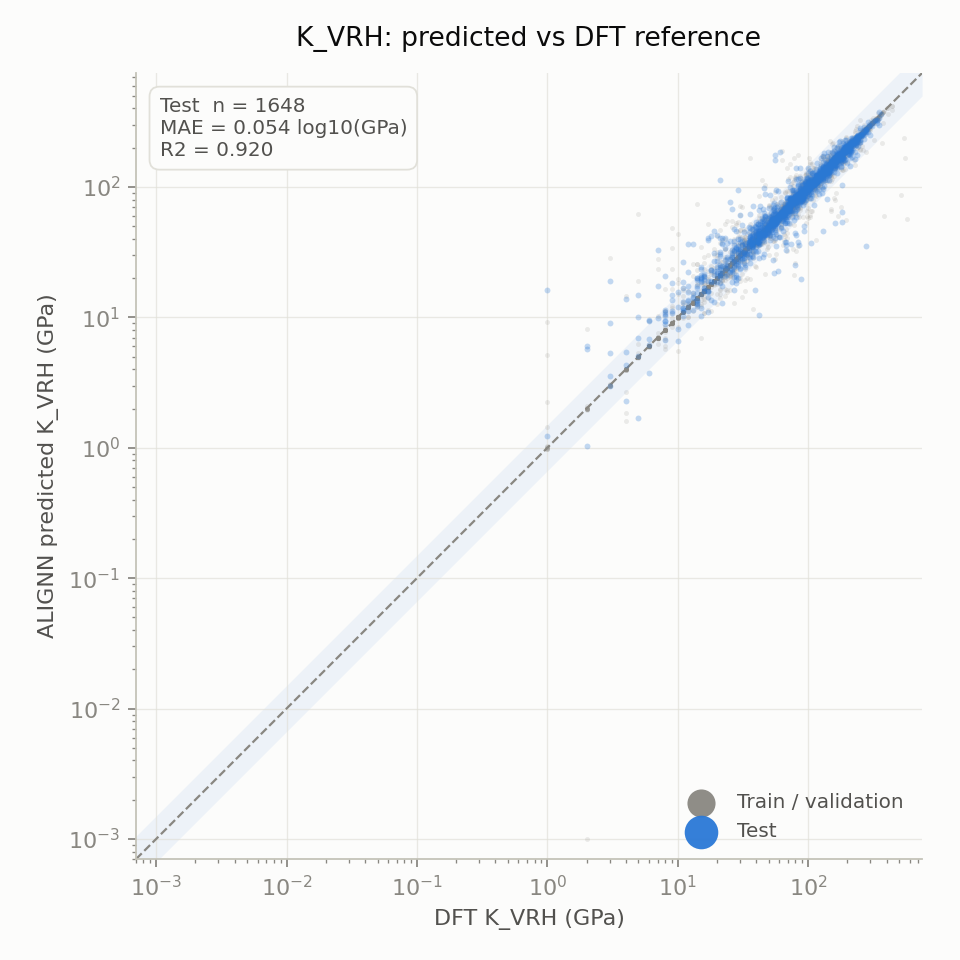
\includegraphics[width=\linewidth]{../results/alignn/parity_K_VRH_alignn.png}
\end{center}
\column{0.49\linewidth}
\begin{center}
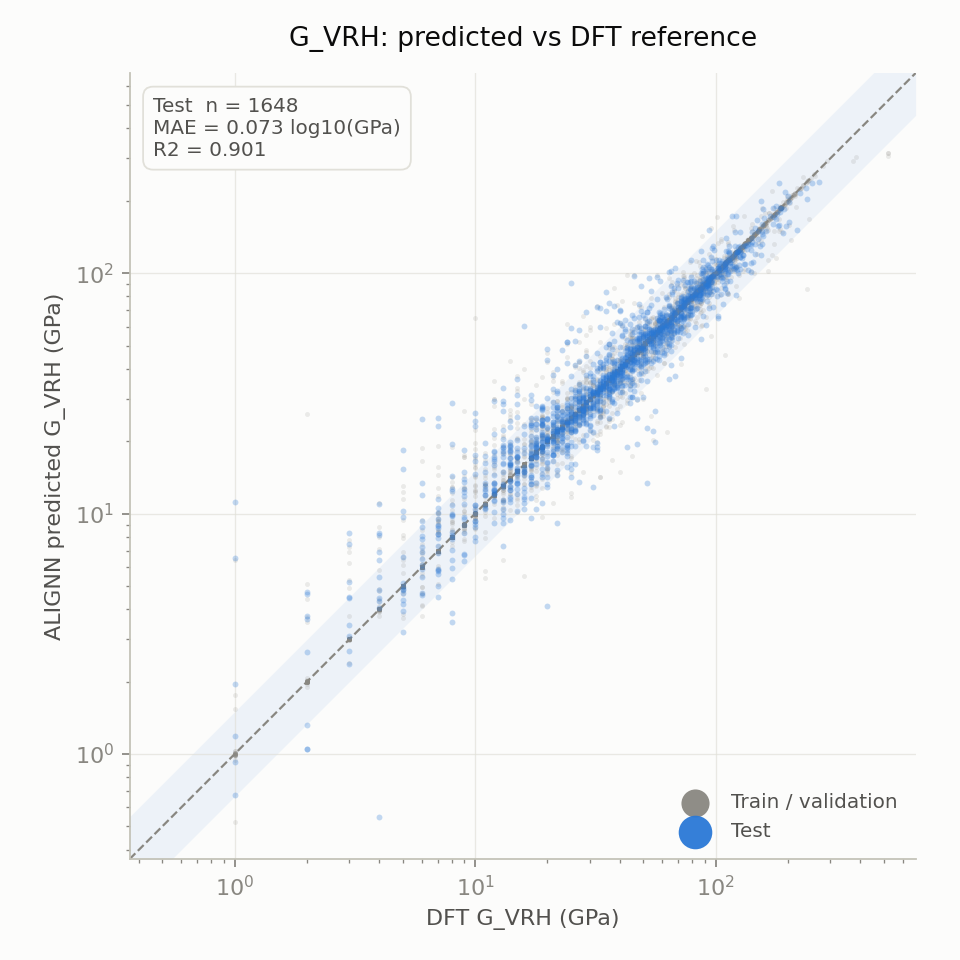
\includegraphics[width=\linewidth]{../results/alignn/parity_G_VRH_alignn.png}
\end{center}
\end{columns}

\vspace{2pt}
{\sffamily\footnotesize
Same crystals, same axes. Bulk: MAE 0.0539, $R^2 = 0.920$. Shear: 0.0725,
$R^2 = 0.901$.

\vspace{2pt}
\textbf{One honest artefact, left visible:} ALIGNN predicted a \emph{negative}
bulk modulus ($-0.57$ GPa) for one soft validation crystal whose true value is
2 GPa. That is a real edge-case failure on soft materials, and it is the reason
the axis is stretched. It was left in rather than clipped.}
\end{frame}

% =============================================================================
\begin{frame}
\SlideHeader{12 \textperiodcentered\ RESULTS}{Where the models fail --- residuals}

\begin{columns}[T]
\column{0.49\linewidth}
\begin{center}
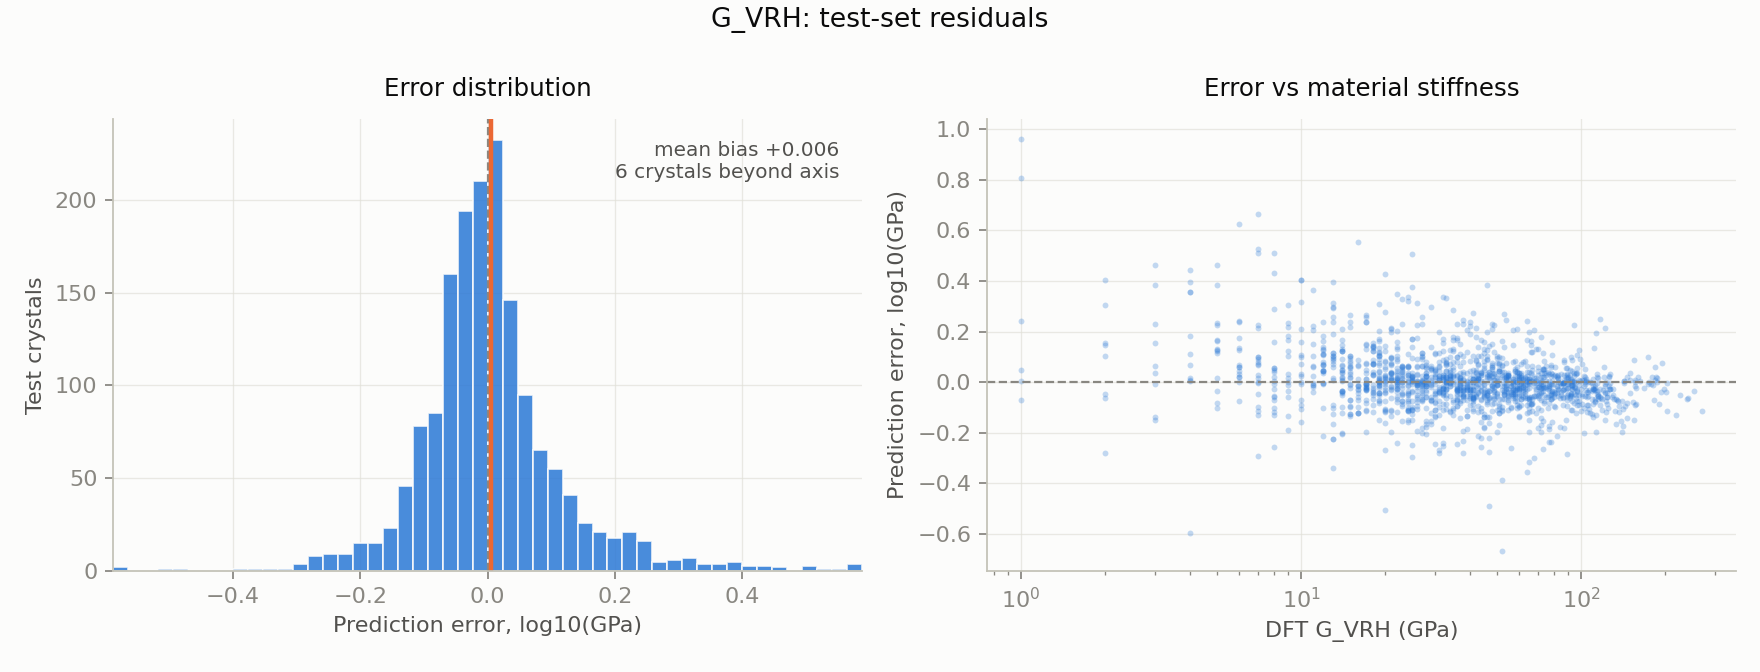
\includegraphics[width=\linewidth]{../results/cgcnn/residuals_G_VRH_ens.png}
\end{center}
{\sffamily\scriptsize\color{Muted}\centering CGCNN ensemble, shear}
\column{0.49\linewidth}
\begin{center}
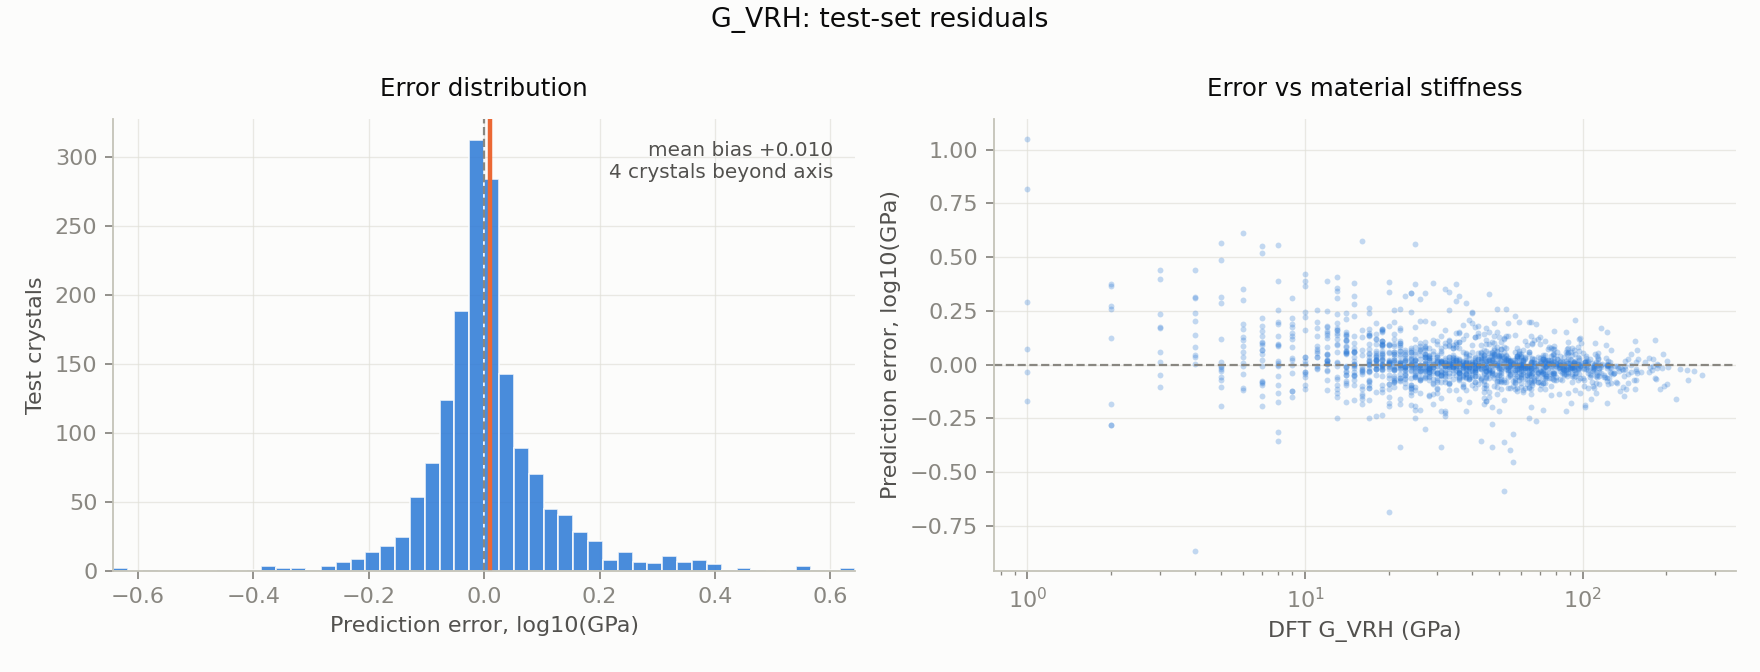
\includegraphics[width=\linewidth]{../results/alignn/residuals_G_VRH_alignn.png}
\end{center}
{\sffamily\scriptsize\color{Muted}\centering ALIGNN, shear}
\end{columns}

\vspace{3pt}
{\sffamily\footnotesize
Residuals fan out below $\sim$30 GPa in both. Stratified by true $\kappa_L$, the
softest quartile has MAE $\log_{10}(G) = 0.134$ against $0.057$ for the
stiffest --- a factor of $2.4$.}

\Takeaway{Both architectures are worst in exactly the regime the screen targets.
Part 7 asks whether that is the model or the labels.}
\end{frame}

% =============================================================================
\begin{frame}
\SlideHeader{13 \textperiodcentered\ RESULTS}{What ensembling buys}

\begin{columns}[T]
\column{0.52\linewidth}
\begin{center}
\includegraphics[width=\linewidth]{figures/ensemble.png}
\end{center}
\column{0.44\linewidth}
{\sffamily\footnotesize
Three models per target, different random initialisations, averaged in
$\log_{10}$ space --- a geometric mean, which is the right notion of middle for
a quantity whose error is proportional.

\vspace{4pt}
Ensembling removed 9--10\% of the error: bulk $\KOneMae \rightarrow \KEnsMae$,
shear $\GOneMae \rightarrow \GEnsMae$.}

\vspace{5pt}
\Card{5.2cm}{CardBg}{CardRule}{%
  \sffamily\footnotesize
  \textbf{And a free uncertainty estimate}\\[3pt]
  The spread across members gives a per-crystal error bar --- the thing PINK's
  single pretrained model cannot produce at all.\\[3pt]
  {\color{SlideAmber}Part 4 shows that estimate is badly overconfident.}}
\end{columns}
\end{frame}

\PartSlide{FOUR}{The physics}{From two moduli to a thermal conductivity}

% =============================================================================

\begin{frame}
\SlideHeader{13b \textperiodcentered\ PHYSICS}{Equations 1--3 --- from moduli to sound}

{\sffamily\scriptsize
The two predicted moduli fix how fast sound travels, and phonon speed sets
thermal conductivity.}

\vspace{3pt}
\begin{align}
v_l &= \sqrt{\frac{K + \tfrac{4}{3}G}{\rho}} &&\text{longitudinal wave speed} \\[2pt]
v_t &= \sqrt{\frac{G}{\rho}} &&\text{transverse wave speed} \\[2pt]
v_s &= \left[\frac{1}{3}\left(\frac{1}{v_l^{3}} + \frac{2}{v_t^{3}}\right)\right]^{-1/3}
   &&\text{averaged sound velocity}
\end{align}

\vspace{2pt}
\begin{center}
{\sffamily\scriptsize
\begin{tabular}{@{}lll@{}}
\toprule
sym & meaning & unit \\
\midrule
$K$, $G$ & bulk, shear modulus \emph{(predicted)} & GPa \\
$\rho$ & mass density \emph{(from the CIF)} & g\,cm$^{-3}$ \\
$v_l, v_t, v_s$ & sound velocities & m\,s$^{-1}$ \\
\bottomrule
\end{tabular}}
\end{center}

\vspace{1pt}
{\sffamily\scriptsize\color{Muted}
Eq.~3 averages three acoustic branches --- one longitudinal, two transverse.}
\end{frame}

\begin{frame}
\SlideHeader{13c \textperiodcentered\ PHYSICS}{Equations 4--6 --- Debye temperature and Gr\"uneisen}

\begin{align}
\Theta_D &= \frac{h}{k_B}\left(\frac{3}{4\pi V}\right)^{1/3} v_s
   &&\text{Debye temperature} \\[2pt]
\nu &= \frac{(v_l/v_t)^2 - 2}{2\,(v_l/v_t)^2 - 2} &&\text{Poisson's ratio} \\[2pt]
\gamma &= \frac{3\,(1 + \nu)}{2\,(2 - 3\nu)} &&\text{Gr\"uneisen parameter}
\end{align}

\vspace{2pt}
\begin{center}
{\sffamily\scriptsize
\begin{tabular}{@{}llllll@{}}
\toprule
sym & meaning & unit & sym & meaning & unit \\
\midrule
$h$ & Planck const. & J\,s & $\Theta_D$ & Debye temp. & K \\
$k_B$ & Boltzmann const. & J\,K$^{-1}$ & $\nu$ & Poisson's ratio & --- \\
$V$ & vol.\ per atom \emph{(CIF)} & \AA$^3$ & $\gamma$ & Gr\"uneisen & --- \\
\bottomrule
\end{tabular}}
\end{center}

\vspace{1pt}
{\sffamily\scriptsize
\textbf{Eq.~6 matters most:} $\gamma$ is \emph{derived} from the same $K$, $G$.}
\end{frame}

\begin{frame}
\SlideHeader{13d \textperiodcentered\ PHYSICS}{Equations 7--8 --- two routes to \texorpdfstring{$\kappa_L$}{kappa}}

\begin{align}
\kappa_L^{\text{Slack}} &=
  \frac{A(\gamma)\,\bar{M}\,V^{1/3}\,\Theta_D^{3}}{\gamma^{2}\,T\,N},
  \qquad A(\gamma) = \frac{2.43\times10^{-8}}{1 - \dfrac{0.514}{\gamma} + \dfrac{0.228}{\gamma^{2}}} \\[3pt]
\kappa_L^{\text{cal}} &= \frac{G\,v_s\,V^{1/3}}{N\,T}\;e^{-\gamma}
  \qquad\text{\sffamily\scriptsize (the boxed equation in the paper's Figure 1)}
\end{align}

\vspace{1pt}
\begin{center}
{\sffamily\scriptsize
\begin{tabular}{@{}llllll@{}}
\toprule
sym & meaning & unit & sym & meaning & unit \\
\midrule
$\bar{M}$ & mean atomic mass & amu & $T$ & temperature, 300 & K \\
$N$ & atoms per cell & --- & $\kappa_L$ & conductivity & W\,m$^{-1}$K$^{-1}$ \\
\bottomrule
\end{tabular}}
\end{center}

\vspace{1pt}
{\sffamily\scriptsize
\textbf{This project reports $\kappa_L^{\text{cal}}$}, whose $\gamma$ dependence
is \emph{exponential}, not $\gamma^{-2}$ --- so swapping $\gamma$ rescales it by
$e^{\gamma_{\text{old}} - \gamma_{\text{new}}}$.}
\end{frame}

\begin{frame}
\SlideHeader{14 \textperiodcentered\ PHYSICS}{The Slack chain --- no free parameters}

\begin{center}
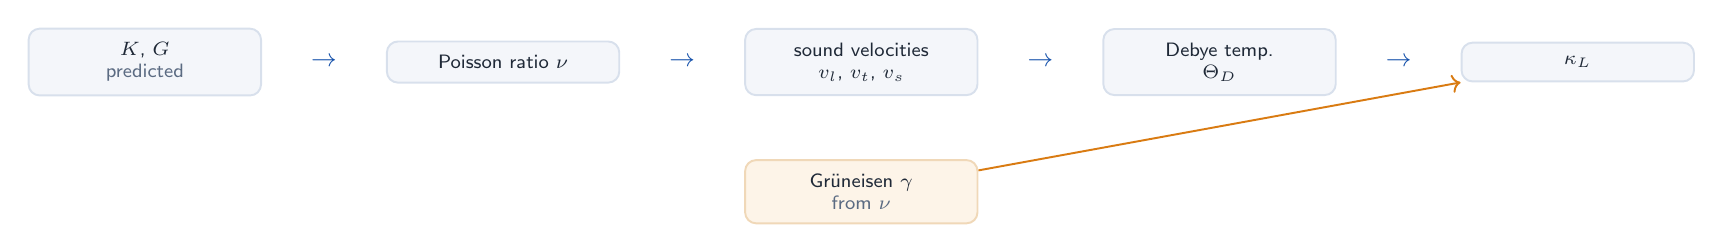
\begin{tikzpicture}[node distance=5mm,
  box/.style={rounded corners=4pt, fill=CardBg, draw=CardRule, line width=0.7pt,
              text width=2.6cm, align=center, inner sep=5pt,
              font=\sffamily\scriptsize\color{SlideInk}},
  arr/.style={font=\color{SlideBlue}\small}]
  \node[box] (b1) {$K$, $G$\\ {\color{Muted}predicted}};
  \node[arr, right=of b1] (a1) {$\rightarrow$};
  \node[box, right=of a1] (b2) {Poisson ratio $\nu$};
  \node[arr, right=of b2] (a2) {$\rightarrow$};
  \node[box, right=of a2] (b3) {sound velocities\\ $v_l$, $v_t$, $v_s$};
  \node[arr, right=of b3] (a3) {$\rightarrow$};
  \node[box, right=of a3] (b4) {Debye temp.\\ $\Theta_D$};
  \node[arr, right=of b4] (a4) {$\rightarrow$};
  \node[box, right=of a4] (b5) {$\kappa_L$};
  \node[box, below=8mm of b3, fill=AmberBg, draw=AmberRule] (g)
       {Gr\"uneisen $\gamma$ \\ {\color{Muted}from $\nu$}};
  \draw[->, SlideAmber, line width=0.7pt] (g) -- (b5.south west);
\end{tikzpicture}
\end{center}

\vspace{2pt}
{\sffamily\footnotesize
Every arrow is a closed-form relation. The only learned quantities in the whole
chain are $K$ and $G$; everything downstream is algebra plus the structural
constants (volume, density, atom count) read straight from the CIF.

\vspace{4pt}
$\gamma$ is \textbf{derived} from the predicted $K/G$ ratio through an empirical
Poisson relation --- matbench contains no measured $\gamma$ at all. That single
choice turns out to dominate several later results.}

\Takeaway{Because the physics is shared and unchanged, any difference between
two of this project's screens is the \emph{moduli}, never the formula.}
\end{frame}

% =============================================================================
\begin{frame}
\SlideHeader{15 \textperiodcentered\ PHYSICS}{The uncertainty interval was badly overconfident}

\begin{columns}[T]
\column{0.52\linewidth}
\begin{center}
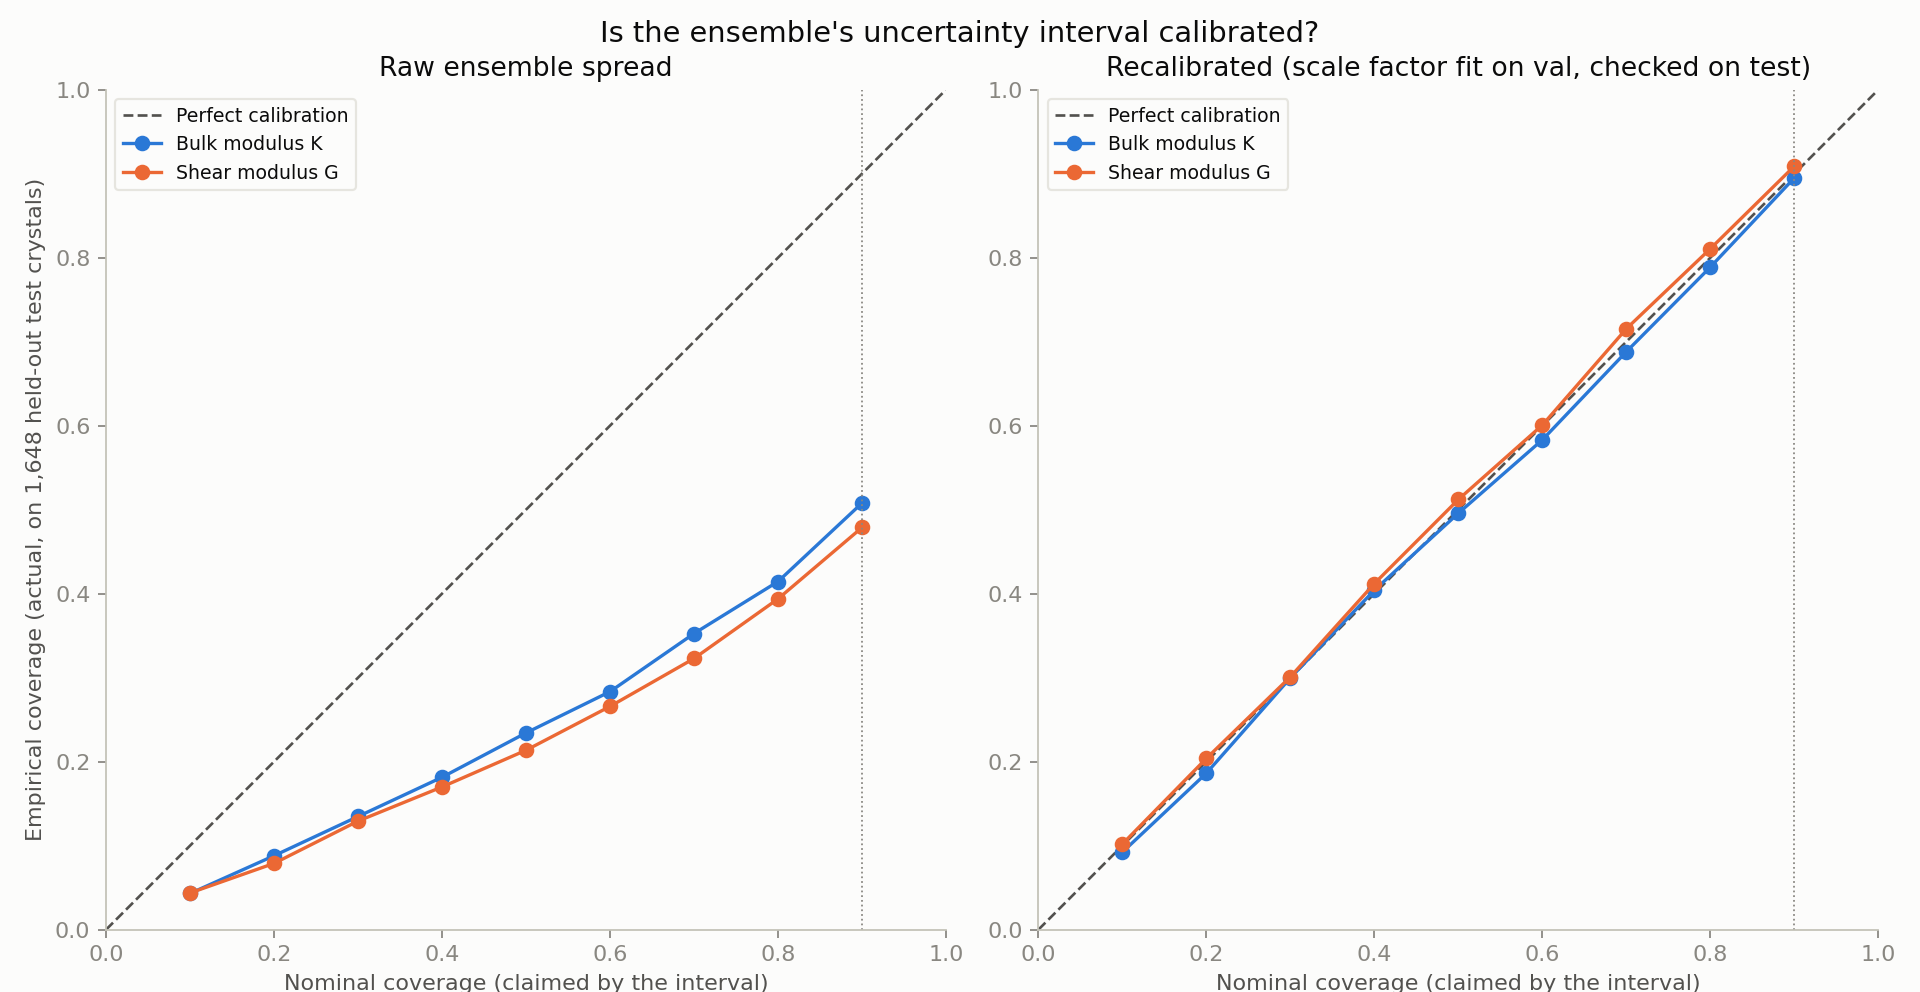
\includegraphics[width=\linewidth]{../results/cgcnn/calibration_check.png}
\end{center}
\column{0.44\linewidth}
{\sffamily\footnotesize
The Monte Carlo p05--p95 band was checked against the test split's real DFT
labels --- no new data needed.}

\vspace{5pt}
\AccentCard{5.2cm}{SlideAmber}{%
  \sffamily\footnotesize
  \textbf{Claimed 90\% coverage. Actual 48--51\%.}\\[3pt]
  Cause: three identically-trained members share blind spots, so member
  \emph{disagreement} runs 4--6$\times$ smaller than true error.}

\vspace{4pt}
{\sffamily\scriptsize
Recalibration factors from validation ($K$ 4.27$\times$, $G$ 4.54$\times$)
recover $\sim$90\% coverage out of sample --- and collapse almost every
``tight'' label on the DFT shortlist to ``wide''.}
\end{columns}

\Takeaway{An ensemble's spread measures variance. The error is bias plus
variance --- and here bias dominates.}
\end{frame}

\PartSlide{FIVE}{Validation against measurement}{45 materials where the answer is known}

% =============================================================================
\begin{frame}
\SlideHeader{16 \textperiodcentered\ REAL DATA}{Measured $\kappa_L$ --- PINK's Figure 6B, our version}

\begin{columns}[T]
\column{0.55\linewidth}
\begin{center}
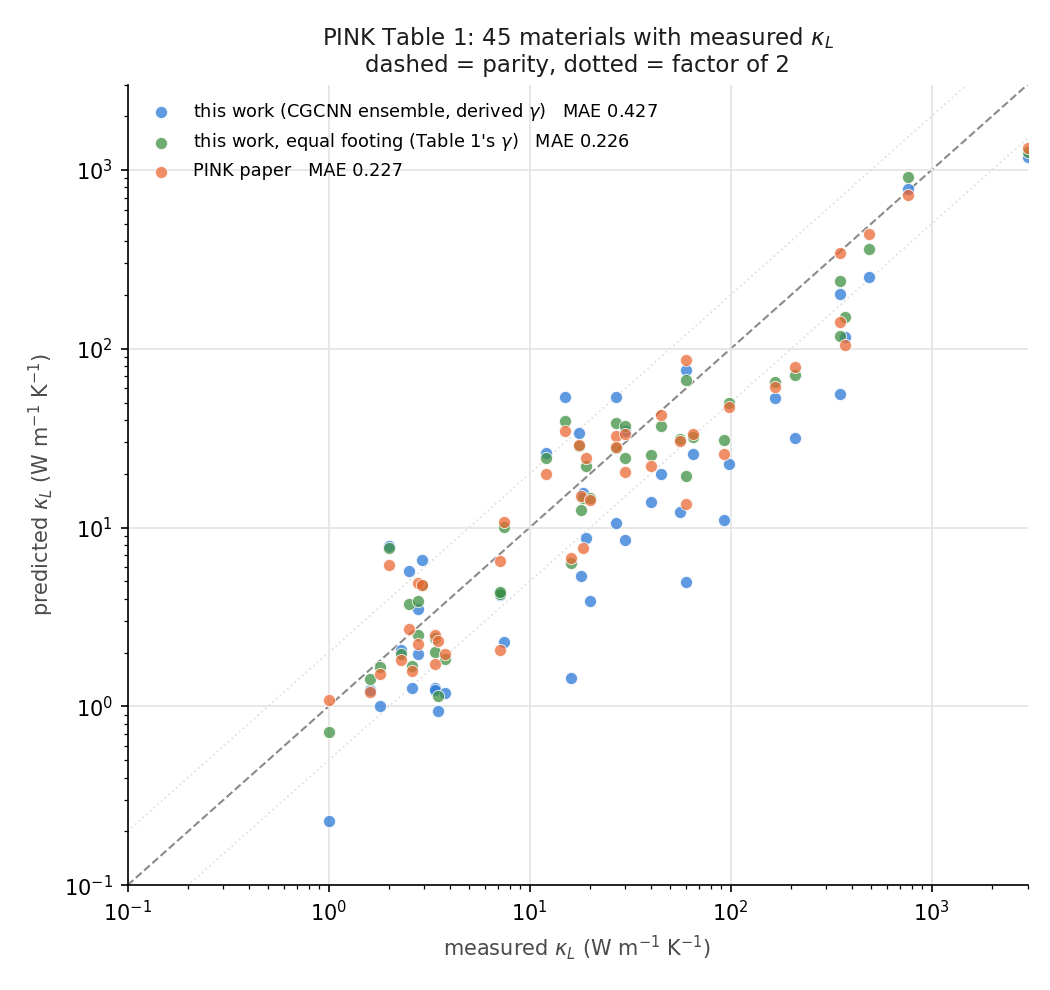
\includegraphics[width=\linewidth]{../results/cgcnn/63_experimental_vs_predicted.png}
\end{center}
\column{0.41\linewidth}
{\sffamily\footnotesize
The paper's Table 1 lists 46 materials with \textbf{experimentally measured}
$\kappa_L$. 45 survive (mp-3490/GaP is deprecated in Materials Project).

\vspace{4pt}
The range spans four orders of magnitude --- AgCl at 1.0 to diamond at 3000
W\,m$^{-1}$K$^{-1}$ --- so everything is scored in $\log_{10}$.}

\vspace{5pt}
\Card{5.0cm}{CardBg}{CardRule}{%
  \sffamily\scriptsize
  \textbf{mean $|\Delta \log_{10}|$}\\[3pt]
  ours, derived $\gamma$ \dotfill 0.427\\
  ours, equal footing \dotfill \textbf{0.226}\\
  the PINK paper \dotfill 0.227}
\end{columns}

\Takeaway{Taken at face value we look twice as bad as the paper. On equal
footing we match it. The next slide is why.}
\end{frame}

% =============================================================================
\begin{frame}
\SlideHeader{17 \textperiodcentered\ REAL DATA}{The comparison was never like-for-like}

\begin{columns}[T]
\column{0.46\linewidth}
{\sffamily\footnotesize
Table 1's $\gamma$ values come from \textbf{AFLOW / experimental lookups} ---
the paper's own text says so. They are \emph{not} produced by the Poisson-ratio
formula that our pipeline uses.

\vspace{4pt}
Neither does the paper's own released screening code use them: it uses the same
formula we do. So comparing our derived $\gamma$ against a looked-up-$\gamma$
table tests \textbf{the $\gamma$ source}, not the model.}

\vspace{5pt}
\Card{5.6cm}{CardBg}{CardRule}{%
  \sffamily\footnotesize
  \textbf{Substituting Table 1's own $\gamma$}\\[3pt]
  changes nothing else --- same moduli, same physics ---\\[2pt]
  $0.427 \rightarrow \mathbf{0.226}$\\[2pt]
  against the paper's $0.227$.}

\column{0.50\linewidth}
\begin{center}
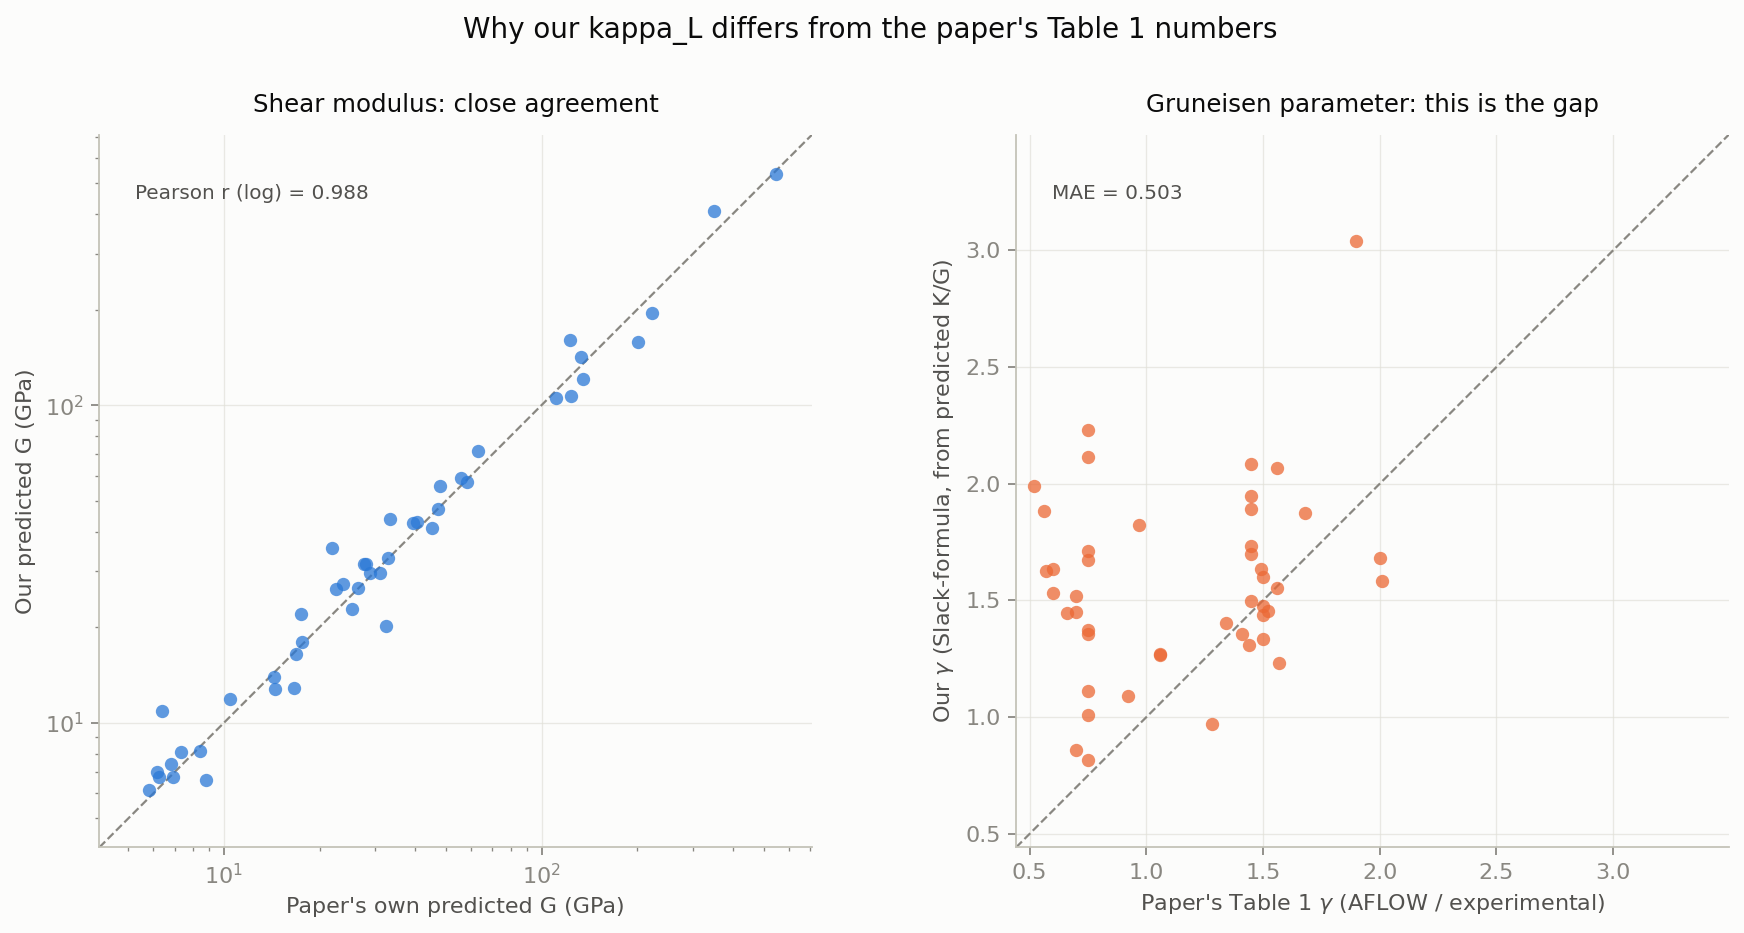
\includegraphics[width=\linewidth]{../results/cgcnn/table1_gamma_diagnostic.png}
\end{center}
{\sffamily\scriptsize\color{Muted}\centering
Our moduli were never the problem: shear modulus and sound velocity agree with
the paper's own tabulated values at $r \approx 0.99$.}
\end{columns}

\Takeaway{This took real investigation to find. It is not something the paper
states, and reporting the 0.427 alone would have been misleading in both
directions.}
\end{frame}

% =============================================================================
\begin{frame}
\SlideHeader{18 \textperiodcentered\ REAL DATA}{The comparison sheet}

\begin{center}
{\sffamily\scriptsize
\begin{tabular}{@{}lrrrr@{}}
\toprule
material & measured & ours (derived $\gamma$) & ours (equal footing) & PINK \\
\midrule
AgCl    &    1.0 &    0.23 &    0.71 &    1.09 \\
Bi$_2$Te$_3$ & 1.6 & 1.24 &   1.43 &    1.20 \\
NaI     &    1.8 &    1.00 &    1.66 &    1.52 \\
PbTe    &    2.5 &    5.72 &    3.74 &    2.71 \\
\midrule
\multicolumn{5}{@{}l@{}}{\color{Muted}\dots\ 37 more \dots} \\
\midrule
AlN     &  350.0 &   55.87 &  118.49 &  140.93 \\
SiC     &  490.0 &  251.19 &  360.10 &  438.31 \\
BN      &  760.0 &  779.67 &  913.63 &  727.98 \\
C (diamond) & 3000.0 & 1180.18 & 1260.63 & 1320.87 \\
\bottomrule
\end{tabular}}
\end{center}

\vspace{3pt}
{\sffamily\footnotesize
\texttt{results/cgcnn/63\_experimental\_vs\_predicted.csv} --- 45 rows,
27 columns. Both $\gamma$ conventions are carried per material, along with each
model's moduli, all three $\gamma$ values, and the p05/p95 interval, so the
choice is visible rather than baked in.}

\Takeaway{ALIGNN is \emph{worse} here --- 0.450 against the CGCNN ensemble's
0.427. It wins on matbench moduli and loses on measured $\kappa_L$. That was
tested, not assumed.}
\end{frame}

% =============================================================================
\begin{frame}
\SlideHeader{19 \textperiodcentered\ REAL DATA}{Two architectures, independently, on the same 1{,}213 crystals}

\begin{columns}[T]
\column{0.52\linewidth}
\begin{center}
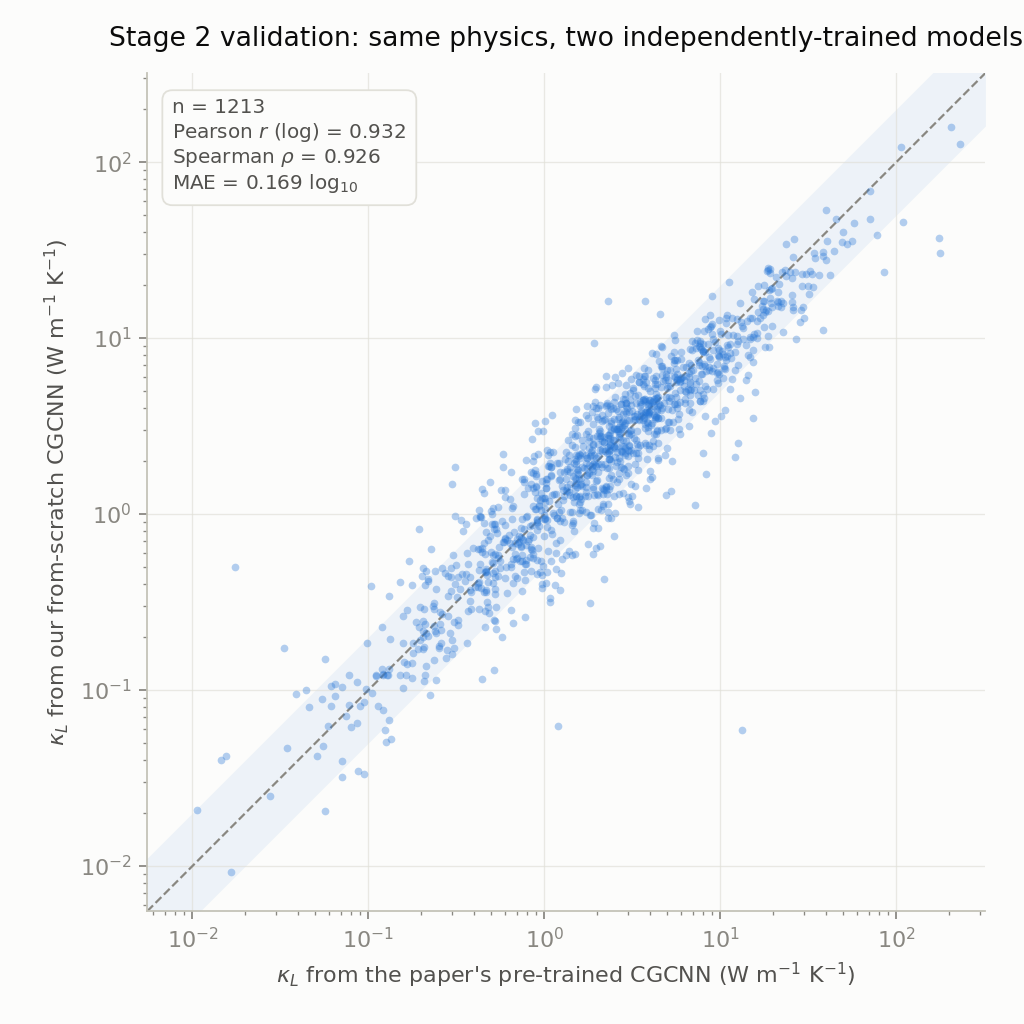
\includegraphics[width=\linewidth]{../results/cgcnn/kappa_validation.png}
\end{center}
\column{0.44\linewidth}
{\sffamily\footnotesize
ALIGNN's moduli pushed through the \emph{unchanged} Slack chain, compared
against the CGCNN ensemble's $\kappa_L$ on the same crystals.

\vspace{4pt}
\textbf{Pearson $r = 0.940$, Spearman $\rho = 0.947$}, MAE 0.141 $\log_{10}$ ---
tighter than CGCNN's own agreement with the paper's pretrained model
($r = 0.932$).}

\vspace{5pt}
\Card{5.2cm}{CardBg}{CardRule}{%
  \sffamily\footnotesize
  Two independently trained architectures, sharing only the data, the split and
  the physics, converging this closely on final $\kappa_L$ is evidence the
  pipeline finds a physical signal rather than architecture-specific noise.}
\end{columns}
\end{frame}

\PartSlide{SIX}{The screen}{554{,}054 materials, scored twice}

% =============================================================================
\begin{frame}
\SlideHeader{20 \textperiodcentered\ THE SCREEN}{The screening funnel --- PINK's Figure 7}

\begin{center}
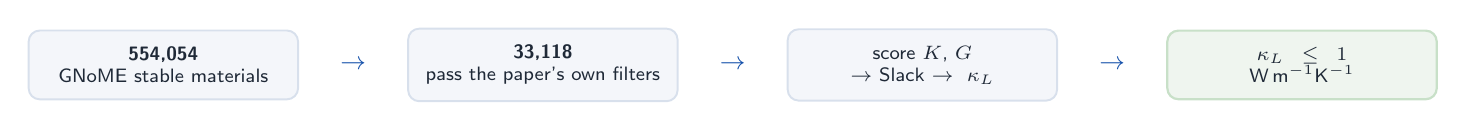
\begin{tikzpicture}[node distance=4mm,
  box/.style={rounded corners=4pt, fill=CardBg, draw=CardRule, line width=0.7pt,
              text width=3.0cm, align=center, inner sep=6pt,
              font=\sffamily\scriptsize\color{SlideInk}},
  hit/.style={rounded corners=4pt, fill=GreenBg, draw=GreenRule, line width=0.8pt,
              text width=3.0cm, align=center, inner sep=6pt,
              font=\sffamily\scriptsize\color{SlideInk}},
  arr/.style={font=\color{SlideBlue}\small}]
  \node[box] (b1) {\textbf{554{,}054}\\ GNoME stable materials};
  \node[arr, right=of b1] (a1) {$\rightarrow$};
  \node[box, right=of a1] (b2) {\textbf{33{,}118}\\ pass the paper's own filters};
  \node[arr, right=of b2] (a2) {$\rightarrow$};
  \node[box, right=of a2] (b3) {score $K$, $G$\\ $\rightarrow$ Slack $\rightarrow \kappa_L$};
  \node[arr, right=of b3] (a3) {$\rightarrow$};
  \node[hit, right=of a3] (b4) {\textbf{$\kappa_L \leq 1$}\\ W\,m$^{-1}$K$^{-1}$};
\end{tikzpicture}
\end{center}

\vspace{4pt}
{\sffamily\footnotesize
The current GNoME snapshot holds \textbf{554{,}054} materials against the
paper's 377{,}221 --- stated explicitly rather than glossed, because it means
the candidate lists are not directly comparable.

\vspace{4pt}
Against the paper's own published 11{,}869 candidates, \textbf{70.8\%} also
appear in our independently derived list. Two pipelines sharing only an
architecture family and a physics formula, on overlapping-but-different
corpora, converging on most of the same discoveries.}

\Takeaway{{\color{SlideAmber}Flagged:} that 70.8\% predates several corrections in
Part 7 and should be recomputed before it is quoted in a paper.}
\end{frame}

% =============================================================================
\begin{frame}
\SlideHeader{21 \textperiodcentered\ THE SCREEN}{What the candidates look like --- PINK's Figure 8}

\begin{columns}[T]
\column{0.49\linewidth}
\begin{center}
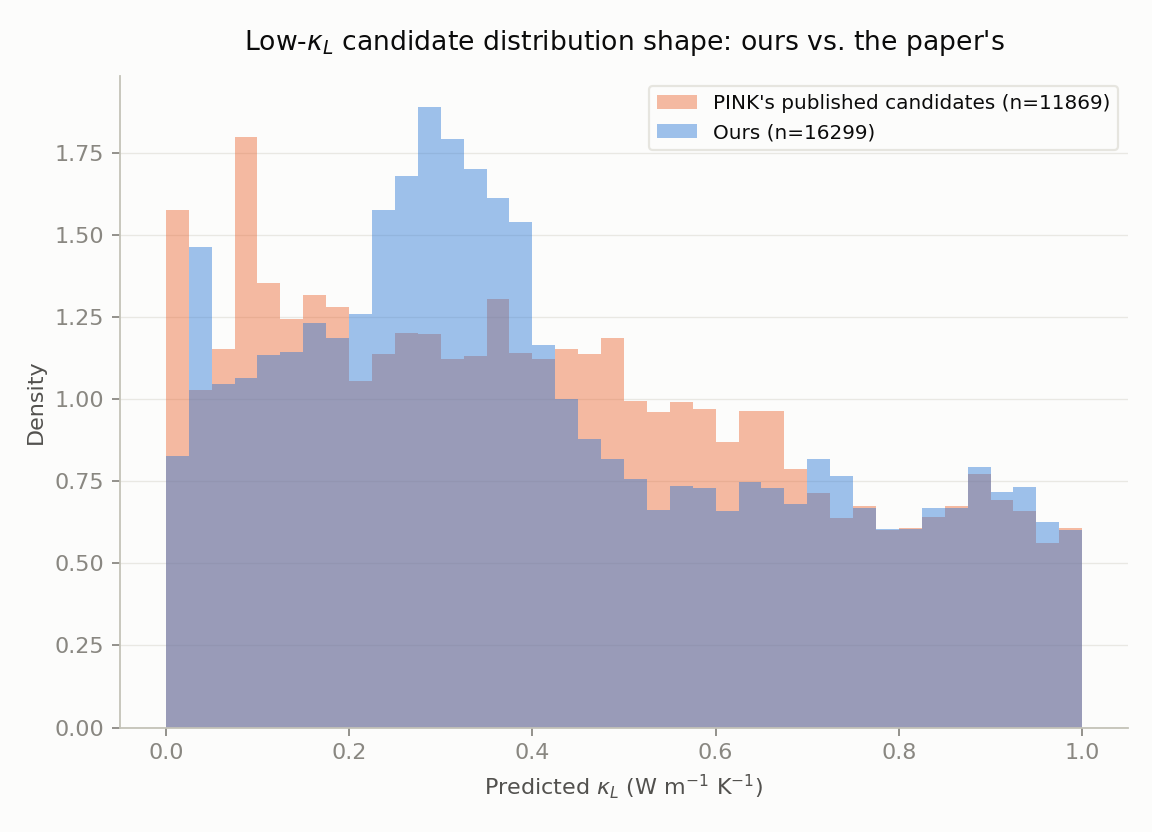
\includegraphics[width=\linewidth]{../results/cgcnn/gnome_kappa_distributions.png}
\end{center}
\column{0.49\linewidth}
\begin{center}
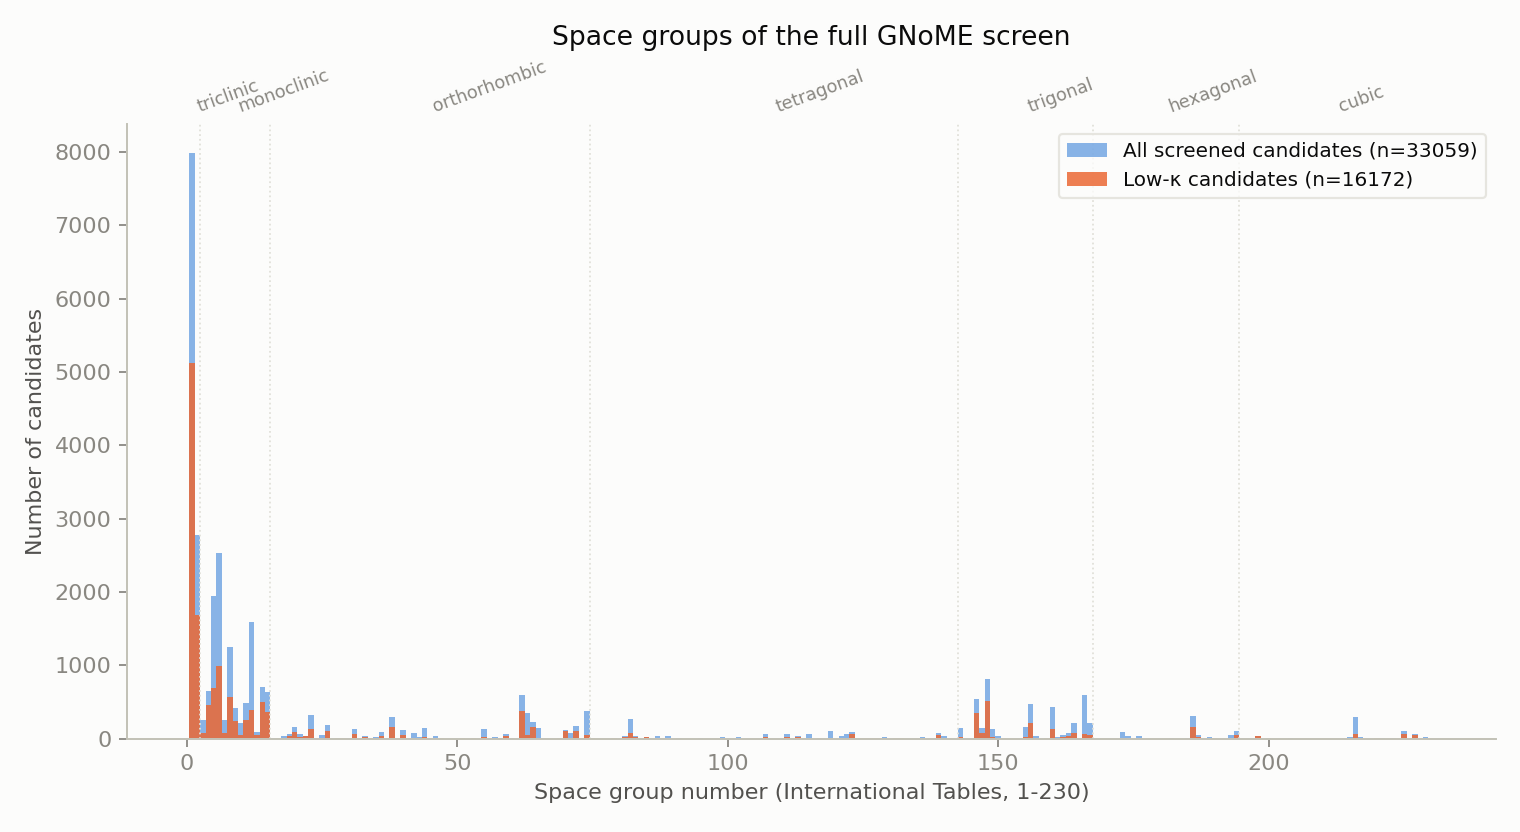
\includegraphics[width=\linewidth]{../results/cgcnn/gnome_screen_spacegroups.png}
\end{center}
\end{columns}

\vspace{2pt}
{\sffamily\scriptsize
$\kappa_L$ distribution and crystal-system breakdown of the screened pool.
Element enrichment tells the clearest physical story: halogens 1.4--1.9$\times$
enriched among low-$\kappa$ candidates, oxygen 0.27$\times$ depleted --- soft
heavy halide lattices against tight oxide bonding.}
\end{frame}

% =============================================================================
\begin{frame}
\SlideHeader{22 \textperiodcentered\ THE SCREEN}{ALIGNN over the whole screen, for the first time}

\begin{columns}[T]
\column{0.52\linewidth}
\begin{center}
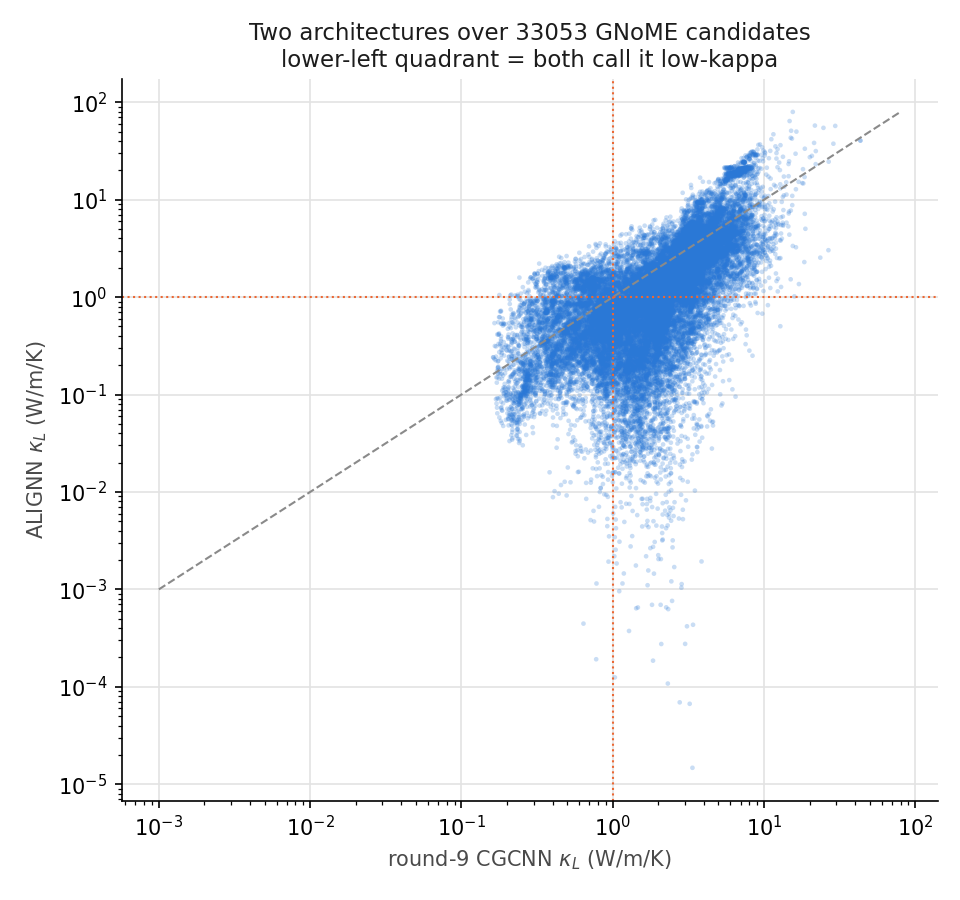
\includegraphics[width=\linewidth]{../results/alignn/57_alignn_vs_r9_gnome.png}
\end{center}
\column{0.44\linewidth}
{\sffamily\footnotesize
All 33{,}118 candidates scored with ALIGNN --- 68 minutes, zero CIF failures.
Only the moduli change; the Slack chain and the structural constants are
identical, so nothing downstream can leak a difference.}

\vspace{5pt}
\Card{5.2cm}{CardBg}{CardRule}{%
  \sffamily\scriptsize
  \textbf{low-$\kappa$ call on 33{,}053 reliable candidates}\\[3pt]
  ALIGNN \dotfill 14{,}711 (44.5\%)\\
  round 9 \dotfill 7{,}262 (22.0\%)\\
  \textbf{both agree} \dotfill \textbf{6{,}006}\\
  Spearman $\rho$ \dotfill 0.723}

\vspace{4pt}
{\sffamily\scriptsize\color{Muted}
65 candidates hit ALIGNN's $\sim$10$^{-3}$ GPa regression floor --- a degenerate
output that reads as a spectacular discovery. Flagged and excluded, not ranked
first.}
\end{columns}
\end{frame}

\PartSlide{SEVEN}{What we found when we checked}{Four evaluation failure modes, and three numbers that were wrong}

% =============================================================================

\begin{frame}
\SlideHeader{22b \textperiodcentered\ THE SCREEN}{The same candidates, four different answers}

\begin{center}
\includegraphics[width=0.84\linewidth]{figures/kappa_dist_all_models.png}
\end{center}

\vspace{-3pt}
{\sffamily\scriptsize
Every model scores the identical 33{,}053 candidates through the identical
physics --- only $K$ and $G$ differ. Low-$\kappa$ counts: \textbf{16{,}130}
(CGCNN), \textbf{14{,}711} (ALIGNN), \textbf{17{,}034} (tree), \textbf{7{,}262}
(round 9). Three agree closely; round 9 sits far right and calls less than half
as many.}
\end{frame}

\begin{frame}
\SlideHeader{22c \textperiodcentered\ THE SCREEN}{Classifying the candidates: elements}

\begin{center}
\includegraphics[width=0.86\linewidth]{figures/elements_all_models.png}
\end{center}

\vspace{-3pt}
{\sffamily\scriptsize
Enrichment is how often candidates containing an element are called
low-$\kappa$, over that model's own base rate. Lines are binned medians.
\textbf{Cs, Rb, K and the halogens Br, Cl, F sit high; O and N sit lowest} ---
which Equations 1--3 predict, since a low $G$ gives a low $v_s$. \textbf{All
four agree on the shape}; round 9 diverges at the electronegative end.}
\end{frame}

\begin{frame}
\SlideHeader{22d \textperiodcentered\ THE SCREEN}{Classifying the candidates: structural families}

\begin{center}
\includegraphics[width=0.88\linewidth]{figures/families_all_models.png}
\end{center}

\vspace{-3pt}
{\sffamily\scriptsize
Non-oxides dominate, but \emph{how} much depends on the model: 68\% (CGCNN),
61\% (ALIGNN), 73\% (tree), 31\% (round 9). \textbf{The family ordering is
stable across all four; the absolute rate is not.}}
\end{frame}

\begin{frame}
\SlideHeader{22e \textperiodcentered\ THE SCREEN}{Every model this project has trained}

\begin{center}
\includegraphics[width=0.80\linewidth]{figures/model_comparison.png}
\end{center}

\vspace{-3pt}
{\sffamily\scriptsize
Bars absent where a model was never trained on that dataset --- not zero, not
measured. \textbf{The composition-only tree beats the CGCNN on AFLOW}
(0.0592 vs 0.1154) while losing on matbench: underfitting, not a limit of graph
networks, since the network's \emph{training} error there (0.103) exceeds the
tree's \emph{test} error.}
\end{frame}

\begin{frame}
\SlideHeader{23 \textperiodcentered\ FINDINGS}{The screening metric was circular}

\begin{columns}[T]
\column{0.52\linewidth}
\begin{center}
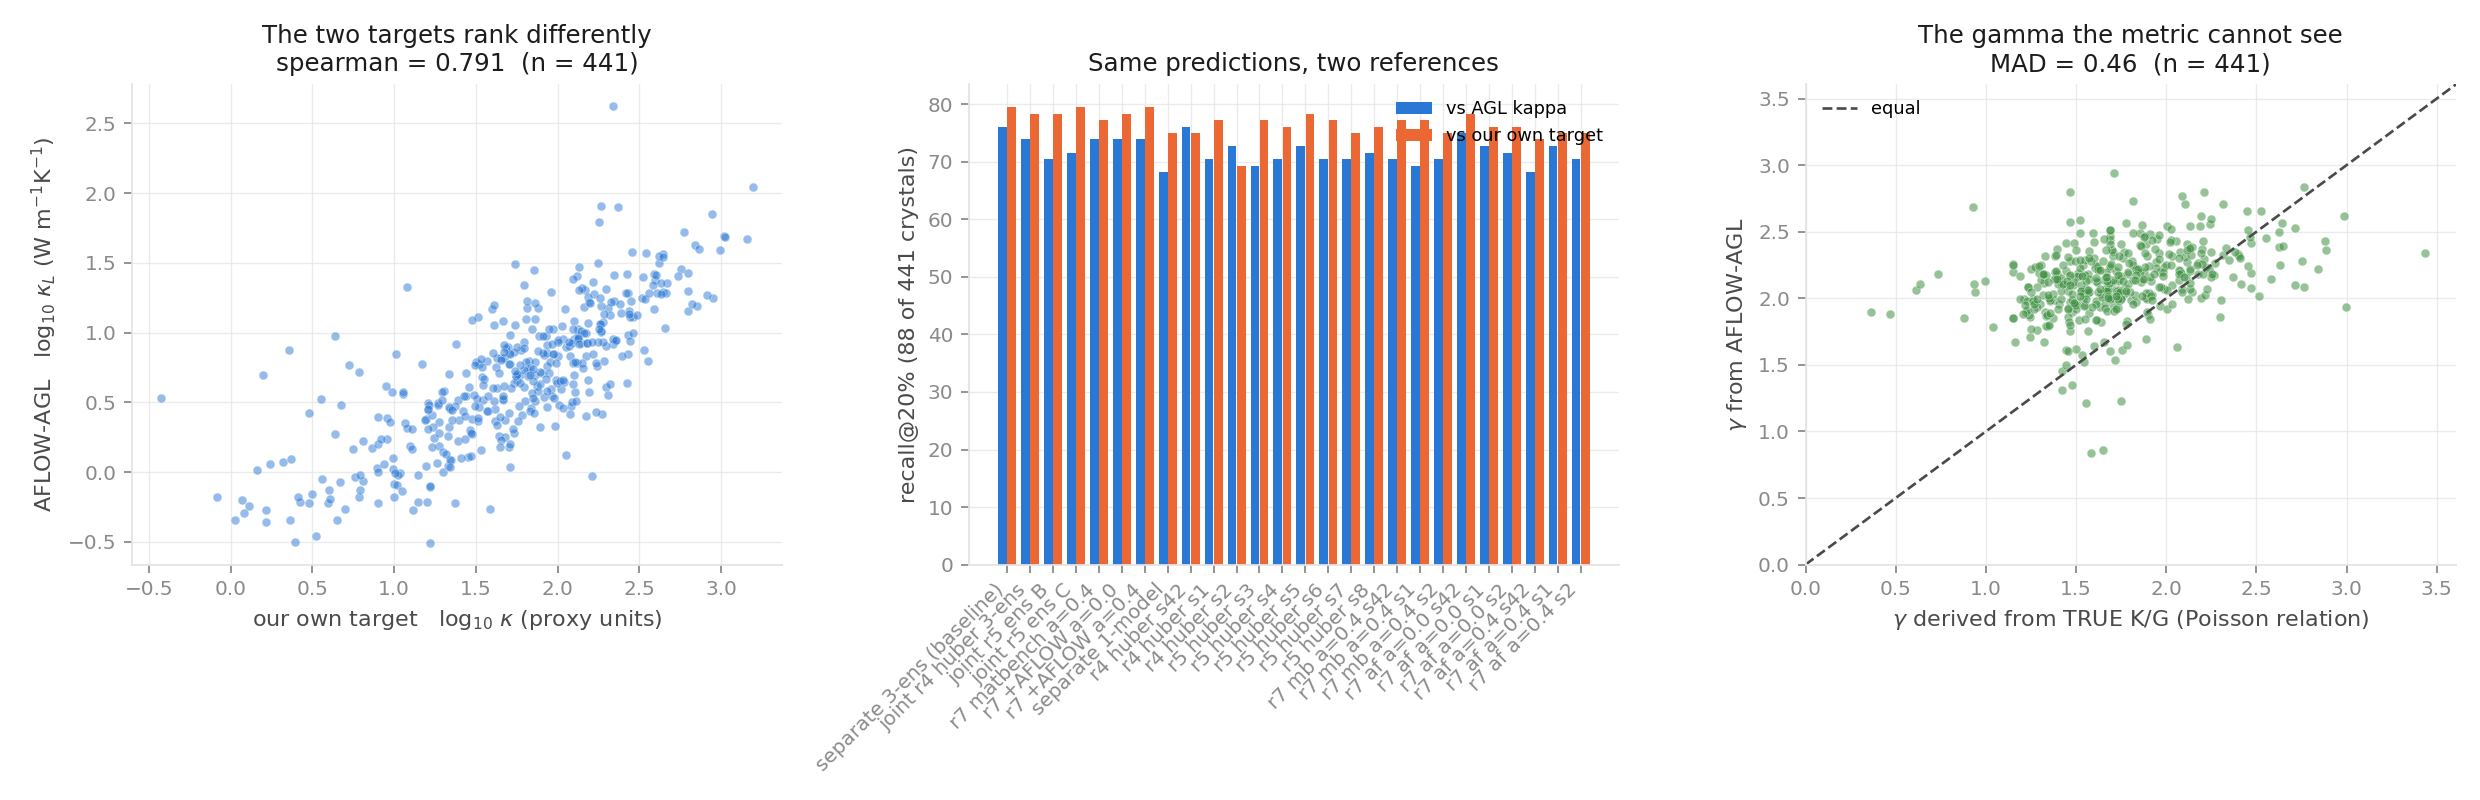
\includegraphics[width=\linewidth]{../results/cgcnn/agl_target/png/48_agl_vs_inhouse_target.png}
\end{center}
\column{0.44\linewidth}
{\sffamily\footnotesize
recall@10\% --- the fraction of the true lowest-$\kappa$ decile recovered ---
was scored against a reference that was \emph{this project's own} Slack chain on
matbench's true moduli, with $\gamma$ derived by the same relation the
prediction side uses.

\vspace{4pt}
Slack cancels. $\gamma$ cancels harder: \textbf{a model predicting a better
$\gamma$ scored worse}.}

\vspace{5pt}
\AccentCard{5.2cm}{SlideAmber}{%
  \sffamily\footnotesize
  Re-scored against AFLOW-AGL's independent $\kappa_L$ (441 matched crystals):
  recall@10\% fell \textbf{20.5 points}, Spearman $\rho$ fell \textbf{0.139}.}
\end{columns}

\Takeaway{The old metric actively penalised the one remaining lever. Quote
Spearman $\rho$ --- it is what transfers between targets ($\rho = 0.92$ across
26 runs); recall@10\% does not ($\rho = 0.20$).}
\end{frame}

% =============================================================================
\begin{frame}
\SlideHeader{24 \textperiodcentered\ FINDINGS}{The misses are a fixed core, not variance}

\begin{columns}[T]
\column{0.52\linewidth}
\begin{center}
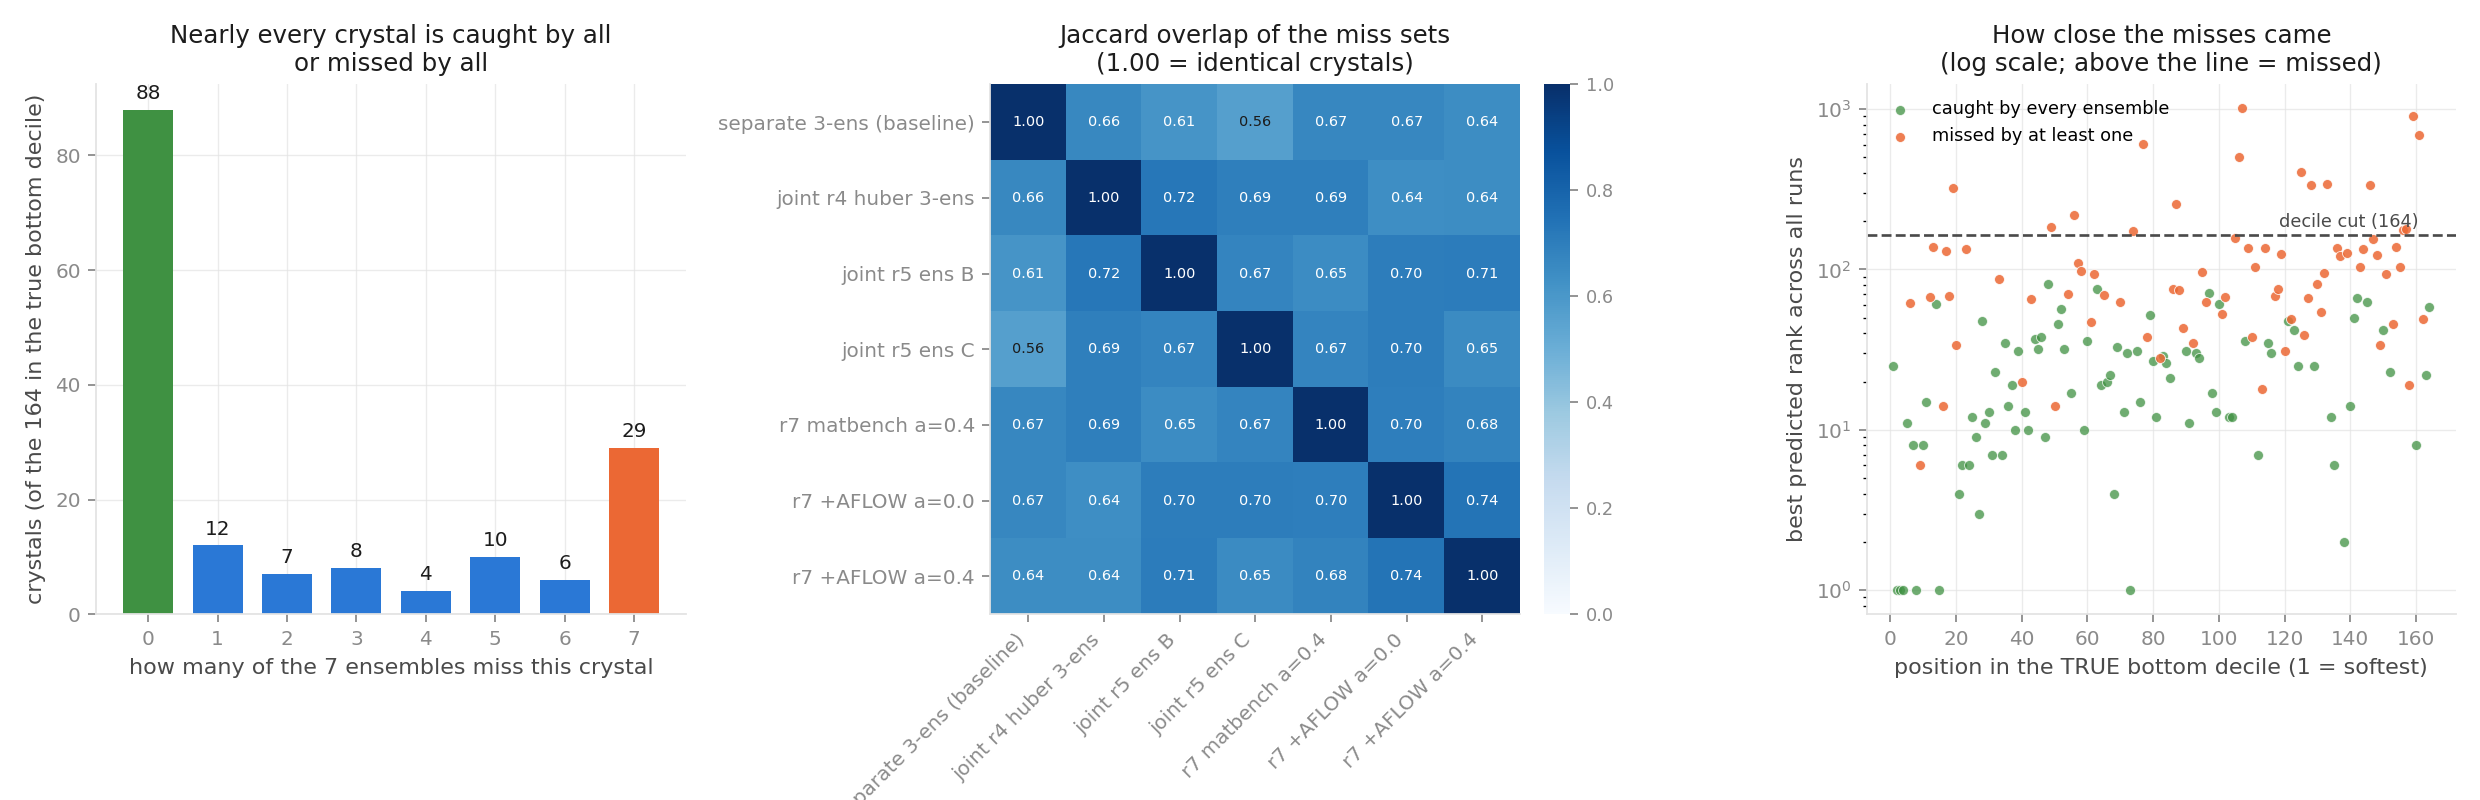
\includegraphics[width=\linewidth]{../results/cgcnn/decile_stability/png/47_missed_decile_stability.png}
\end{center}
\column{0.44\linewidth}
{\sffamily\footnotesize
Fingerprinting the saved prediction vectors collapsed 34 roster entries to
\textbf{26 distinct} runs --- eight were byte-identical duplicates.

\vspace{4pt}
Across those 26, recall spans \textbf{64.0--70.7\%}. \emph{Which} crystals are
missed is remarkably stable: \textbf{16 missed by all 26 runs}, 29 by all seven
ensembles, 65 never missed.}

\vspace{5pt}
\Card{5.2cm}{CardBg}{CardRule}{%
  \sffamily\scriptsize
  The 16 permanent misses: TmAg$_3$, MgAgAs, CeTe, Cs$_2$NaAlH$_6$, InSb, YSe
  and ten others --- median 4 sites, 9 of 16 cubic, never ranked better than
  173rd by anything.}
\end{columns}

\Takeaway{The ceiling is in the inputs, not the architecture. Seven rounds of
architecture work never moved it.}
\end{frame}

% =============================================================================
\begin{frame}
\SlideHeader{25 \textperiodcentered\ FINDINGS}{A composition-only tree beats the network}

\begin{columns}[T]
\column{0.50\linewidth}
\begin{center}
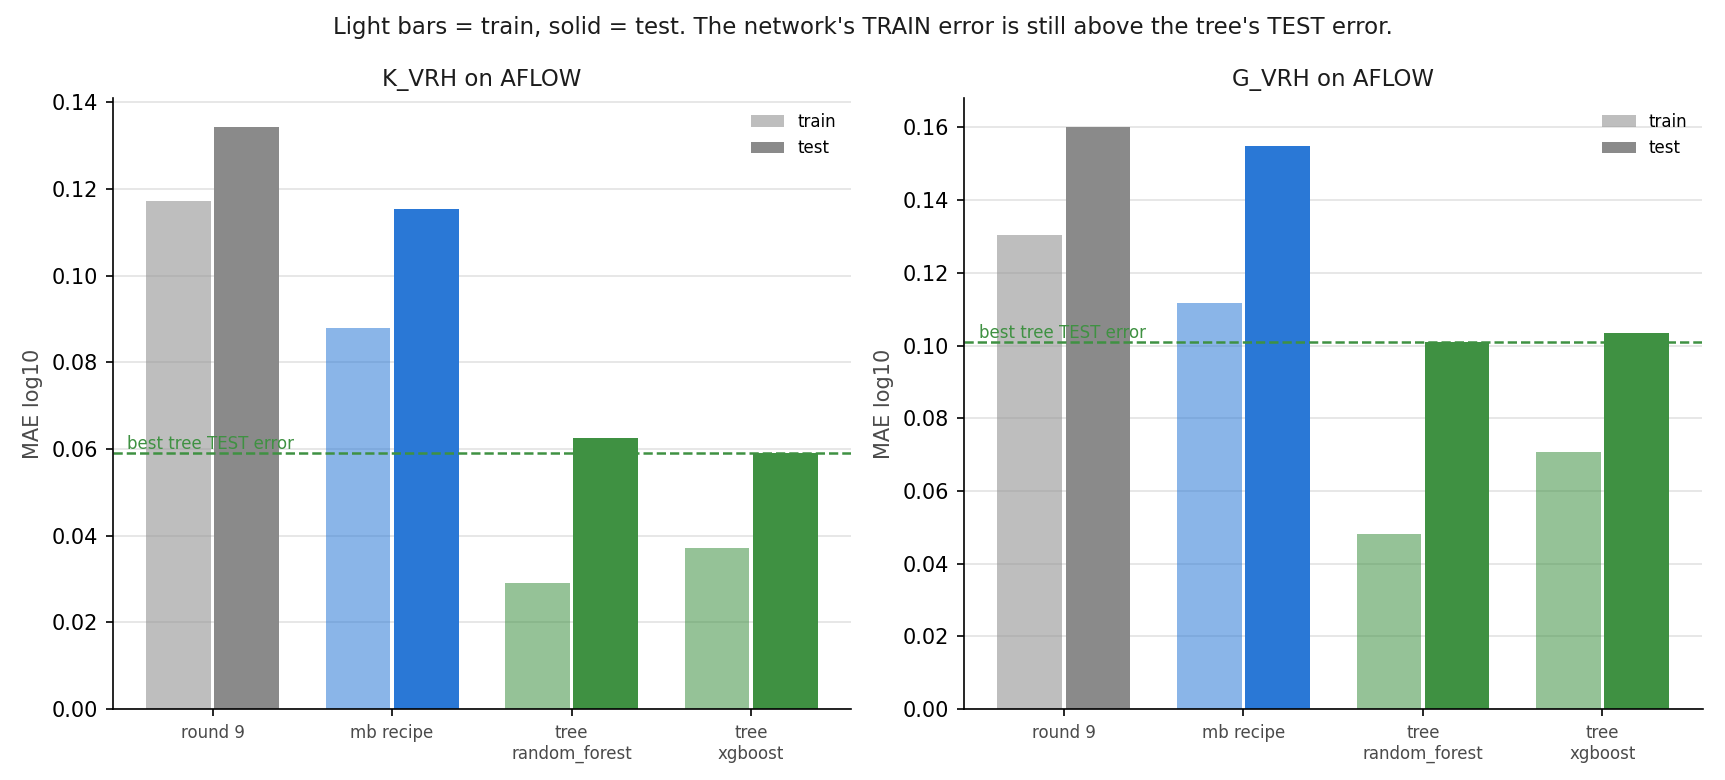
\includegraphics[width=\linewidth]{../results/cgcnn/underfitting/png/53_underfitting_verdict.png}
\end{center}
\column{0.46\linewidth}
{\sffamily\footnotesize
A decision tree on the composition-weighted mean of the same 92-dim element
table --- \textbf{no structure, no bonds} --- on the identical split:}

\vspace{4pt}
{\sffamily\scriptsize
\begin{tabular}{@{}lrr@{}}
\toprule
$K$ MAE $\log_{10}$ & tree & CGCNN \\
\midrule
matbench & 0.0868 & \textbf{0.0696} \\
AFLOW    & \textbf{0.0592} & 0.1154 \\
\bottomrule
\end{tabular}}

\vspace{5pt}
\AccentCard{5.2cm}{SlideAmber}{%
  \sffamily\footnotesize
  \textbf{The cause is underfitting, checked directly.}\\[3pt]
  Round 9's \emph{training} error on AFLOW $K$ is 0.103 --- worse than the
  tree's \emph{test} error of 0.059. A model that cannot fit its own training
  data is not out-generalised.}
\end{columns}

\Takeaway{Never report ``a decision tree beat our GNN'' without saying the GNN
was underfit. Composition memorisation was ruled out: only 9.6\% of AFLOW test
formulas appear in train, and excluding them moves the MAE by $<0.003$.}
\end{frame}

% =============================================================================
\begin{frame}
\SlideHeader{26 \textperiodcentered\ FINDINGS}{The label noise everyone quotes was the wrong number}

\begin{columns}[T]
\column{0.55\linewidth}
\begin{center}
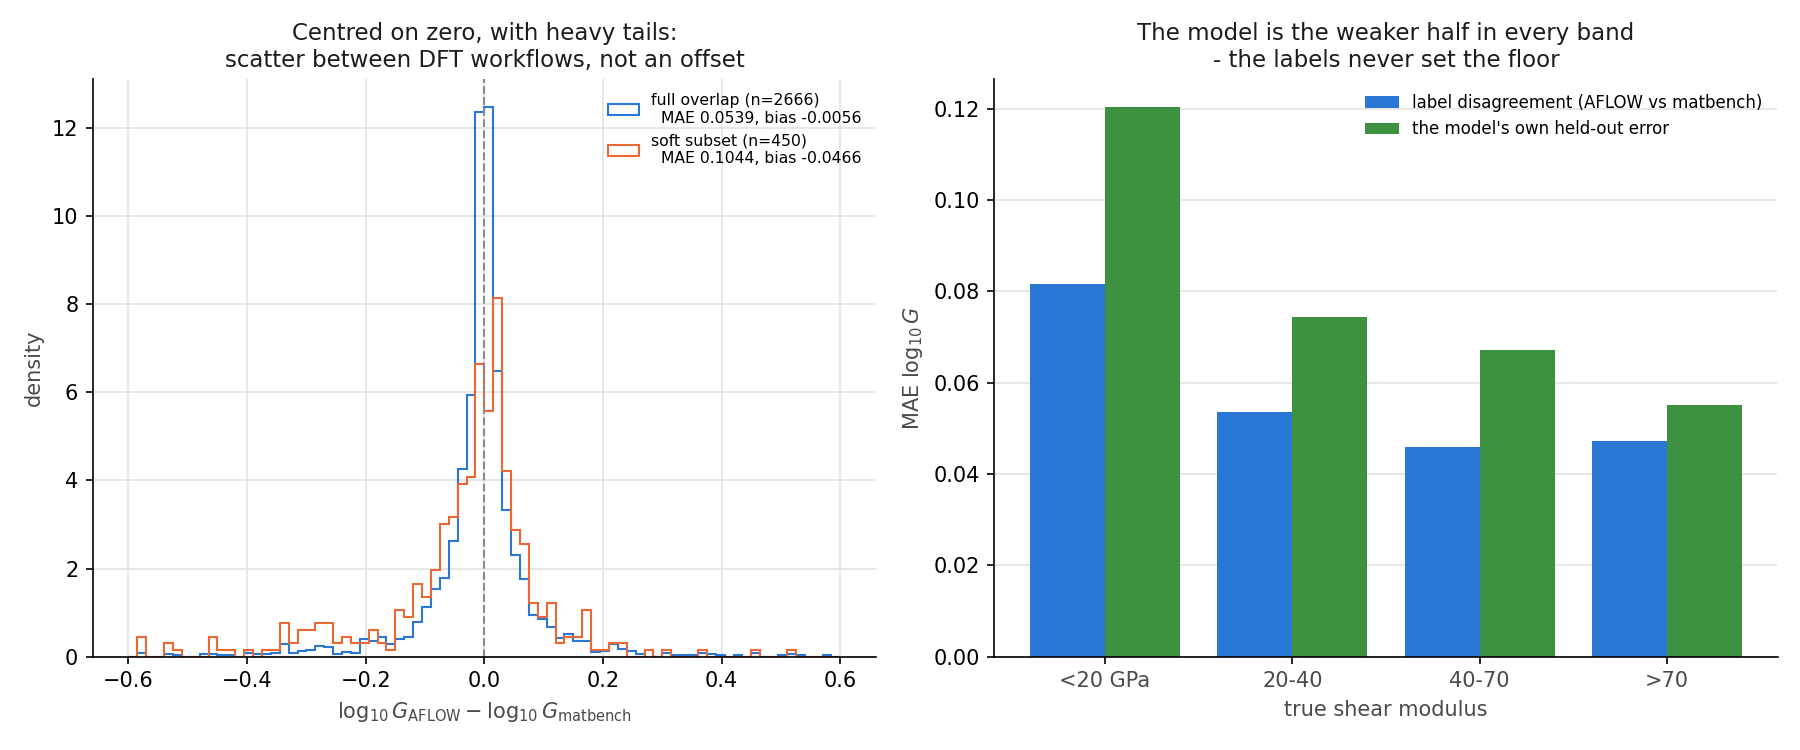
\includegraphics[width=\linewidth]{../results/cgcnn/59_cross_source_label_noise.png}
\end{center}
\column{0.41\linewidth}
{\sffamily\footnotesize
A single constant --- $|\Delta \log_{10} G| = 0.1085$ --- was hard-coded into
four scripts as \emph{the} matbench/AFLOW label noise, and divided by a
whole-test-set model error to argue the labels set the accuracy floor.}

\vspace{5pt}
\AccentCard{5.0cm}{SlideAmber}{%
  \sffamily\scriptsize
  \textbf{0.1085 is the \emph{soft subset's} number.}\\[3pt]
  Full overlap (n = 2{,}666): \textbf{0.0539}\\[2pt]
  Population-matched ratio: 0.69, not 1.39\\[2pt]
  Per stiffness band the \emph{model's} error exceeds the label disagreement in
  \textbf{all four}.}

\vspace{4pt}
{\sffamily\scriptsize
Also: the soft subset's apparent offset is a \emph{selection artefact} --- the
bias flips sign depending on which source did the selecting.}
\end{columns}

\Takeaway{The network, not the labels, is the weaker half --- so there is real
headroom left. And ``AEL vs VRH'' is not a convention difference: both sources
report VRH.}
\end{frame}

% =============================================================================
\begin{frame}
\SlideHeader{27 \textperiodcentered\ FINDINGS}{Where a cross-model disagreement actually lives}

\begin{columns}[T]
\column{0.56\linewidth}
\begin{center}
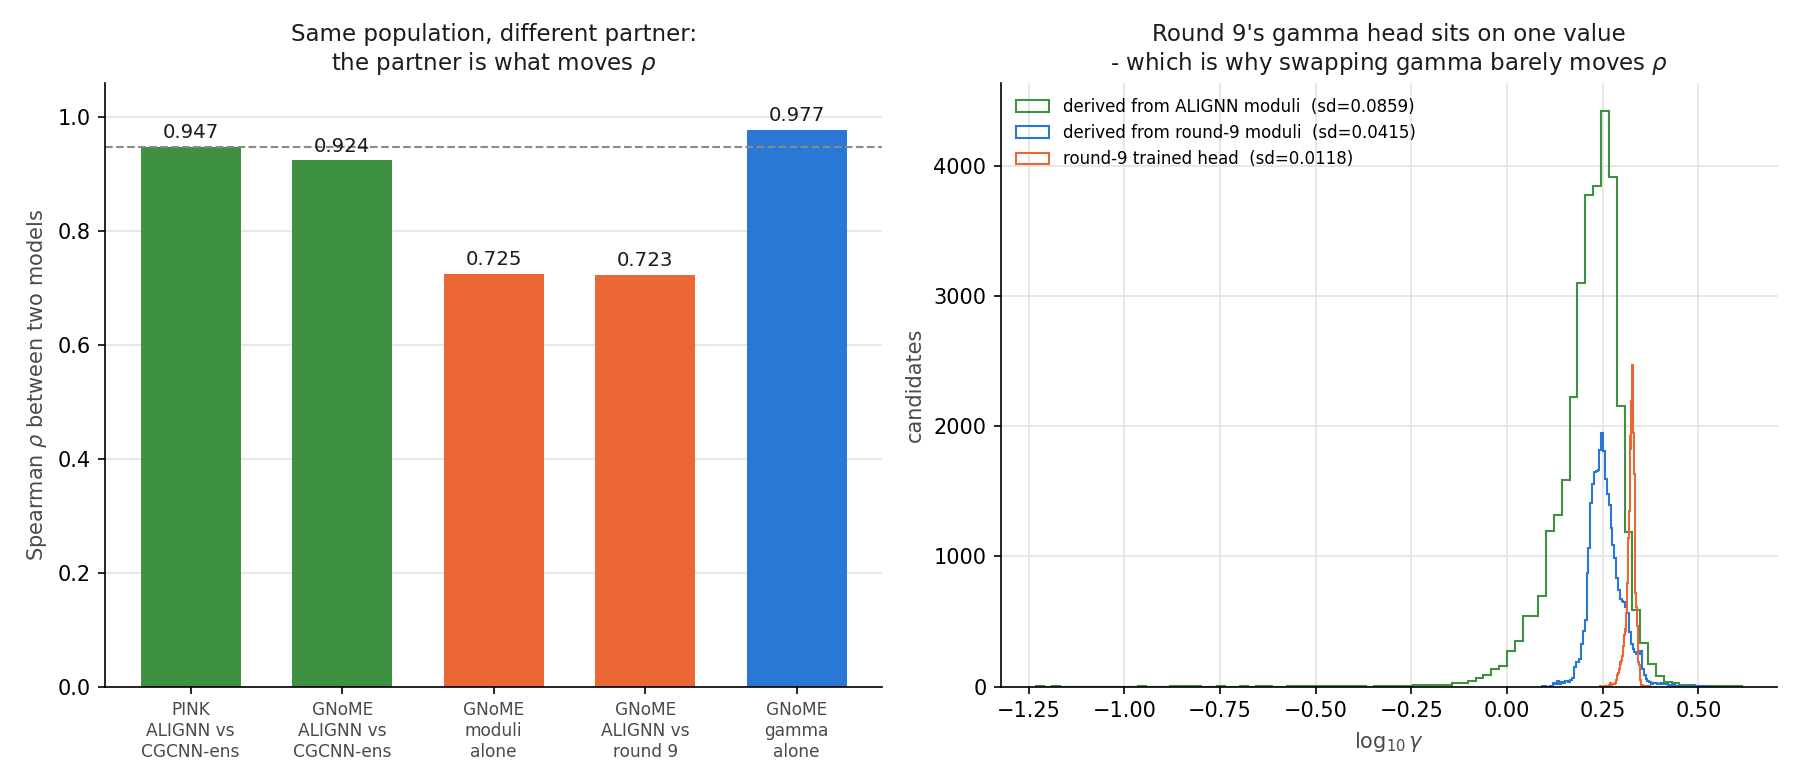
\includegraphics[width=\linewidth]{../results/alignn/58_rho_decomposition.png}
\end{center}
\column{0.40\linewidth}
{\sffamily\footnotesize
Agreement between ALIGNN and the CGCNN ensemble is $\rho = 0.947$ on the PINK
set but only 0.723 against round 9 on GNoME. Two explanations were plausible:
the exotic GNoME chemistry, or the partner model.}

\vspace{5pt}
{\sffamily\scriptsize
\begin{tabular}{@{}lr@{}}
\toprule
population cost (PINK $\rightarrow$ GNoME) & $-0.023$ \\
partner cost (ens.\ $\rightarrow$ round 9) & $\mathbf{-0.201}$ \\
\midrule
moduli alone & 0.725 \\
$\gamma$ alone & 0.977 \\
\bottomrule
\end{tabular}}

\vspace{4pt}
{\sffamily\scriptsize\color{Muted}
Holding the partner fixed, GNoME's chemistry costs almost nothing. Swapping the
partner costs nine times more --- and it is entirely the moduli.}
\end{columns}

\Takeaway{Round 9's $\gamma$ head collapsed to near-constant (sd
$0.0118$, rank correlation $-0.028$). A constant barely perturbs a
\emph{ranking} --- invisible to $\rho$, still wrong in absolute $\kappa$.}
\end{frame}

% =============================================================================
\begin{frame}
\SlideHeader{28 \textperiodcentered\ FINDINGS}{The joint model worked better than the record said}

\begin{columns}[T]
\column{0.55\linewidth}
\begin{center}
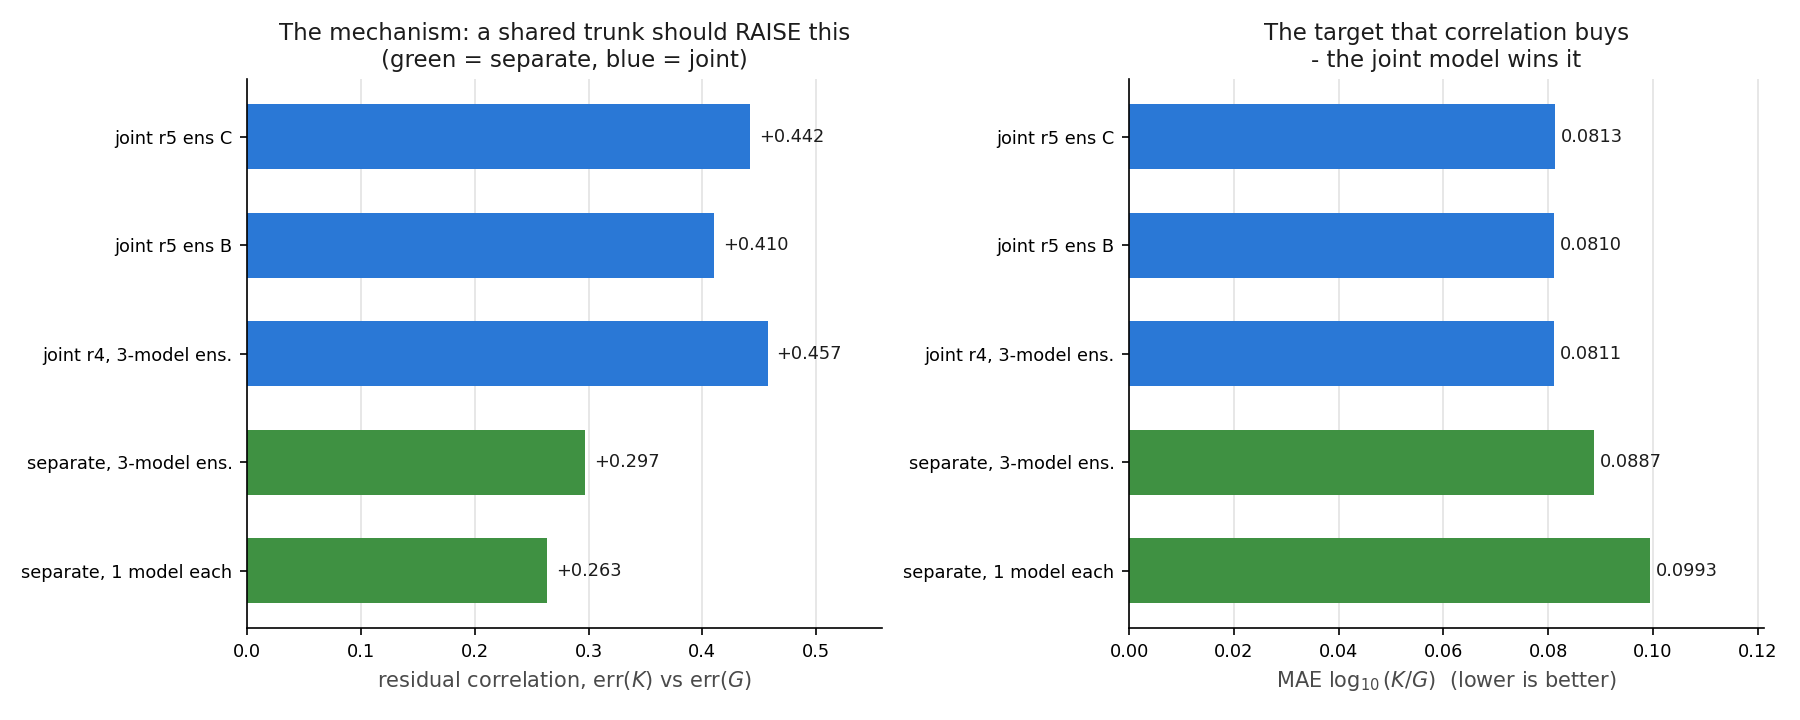
\includegraphics[width=\linewidth]{../results/cgcnn/60_residual_corr_table.png}
\end{center}
\column{0.41\linewidth}
{\sffamily\footnotesize
$\kappa_L$ depends on $K$ and $G$ only through their \emph{ratio}, and in log
space a ratio is a difference --- so independent errors \textbf{add}. A shared
trunk should make them correlate instead.}

\vspace{4pt}
{\sffamily\scriptsize
\begin{tabular}{@{}lrr@{}}
\toprule
& corr & MAE $\log_{10}(K/G)$ \\
\midrule
separate, 1 each & $+0.263$ & 0.0993 \\
separate, 3-ens  & $+0.297$ & 0.0887 \\
\textbf{joint 3-ens} & $\mathbf{+0.457}$ & \textbf{0.0811} \\
\bottomrule
\end{tabular}}

\vspace{4pt}
{\sffamily\scriptsize\color{Muted}
A published table had labelled the first two columns ``separate'' and
``joint'' --- so it contained no joint model at all. The real correlation is
1.5$\times$ the ensemble's.}
\end{columns}

\Takeaway{The mechanism worked, and is paid for in per-modulus accuracy ---
the two nearly cancel in $\kappa_L$ (0.1868 vs 0.1897).}
\end{frame}

\PartSlide{EIGHT}{What happens next}{The one experiment that closes the gap}

% =============================================================================
\begin{frame}
\SlideHeader{29 \textperiodcentered\ NEXT}{The missing piece --- and the experiment for it}

{\sffamily\footnotesize
Every result in this project is model-vs-model or model-vs-database. \textbf{No
candidate has ever been checked against a calculation we ran ourselves.} That is
the single thing blocking any discovery claim.}

\vspace{5pt}
\begin{columns}[T]
\column{0.31\linewidth}
\AccentCard{3.6cm}{SlideGreen}{%
  \sffamily\scriptsize
  \textbf{Arm A --- consensus low}\\[3pt]
  All four models agree. Ranked by the \emph{most pessimistic} of them, not the
  lowest prediction.\\[3pt]
  8 of 69 eligible}
\column{0.31\linewidth}
\AccentCard{3.6cm}{SlideAmber}{%
  \sffamily\scriptsize
  \textbf{Arm B --- adjudication}\\[3pt]
  Three models say low, round 9 says high. GNoME has no ground truth; DFT
  settles it.\\[3pt]
  6 of 214 eligible}
\column{0.31\linewidth}
\AccentCard{3.6cm}{Muted}{%
  \sffamily\scriptsize
  \textbf{Arm C --- negative control}\\[3pt]
  All four call it stiff. Without this, a confirmed Arm A means little.\\[3pt]
  4 of 297 eligible}
\end{columns}

\vspace{6pt}
{\sffamily\footnotesize
\textbf{Compute the elastic tensor, not $\kappa$.} Two independent diagnostics
localise every model disagreement here to the moduli, and a finite-strain
elastic tensor on a 6--10 atom cell is a handful of static calculations.
Quasi-harmonic Debye $\kappa$ then follows from the same tensor almost free.

\vspace{3pt}
\textbf{Start with MoBr$_5$Cl} --- 7 atoms, $Cm$, and the sharpest disagreement
in the whole screen: ALIGNN 0.028 against round 9's 4.524, a factor of 162.}
\end{frame}

% =============================================================================

\begin{frame}
\SlideHeader{29b \textperiodcentered\ NEXT}{The 18 materials, and what each arm asks}

\begin{center}
\includegraphics[width=0.84\linewidth]{figures/dft_validation_set.png}
\end{center}

\vspace{-3pt}
{\sffamily\scriptsize
Four models per material, all cells $\leq$ 10 atoms. Amber band = the
adjudication arm, where three models say low and round 9 says high --- only DFT
settles those. Green = consensus low, grey = negative control. Start with
\textbf{MoBr$_5$Cl}: ALIGNN 0.028 against round 9's 4.524, the sharpest
disagreement in the screen.}
\end{frame}

\begin{frame}
\SlideHeader{30 \textperiodcentered\ NEXT}{Where this can be published}

\begin{columns}[T]
\column{0.48\linewidth}
{\sffamily\footnotesize
The honest framing is a \textbf{reproducibility and evaluation paper}, not a
materials-discovery paper. The contribution is a set of measured failure modes
that inflate reported performance in this problem class:}

\vspace{4pt}
{\sffamily\footnotesize
\textbf{1.} a circular screening metric\\
\textbf{2.} uncalibrated ensemble intervals\\
\textbf{3.} a composition baseline beating an underfit GNN\\
\textbf{4.} population-dependent label noise}

\column{0.48\linewidth}
\AccentCard{5.6cm}{SlideAmber}{%
  \sffamily\footnotesize
  \textbf{What blocks the discovery framing}\\[3pt]
  No external validation --- fixed by Arm B above.\\[3pt]
  No net improvement: seven rounds produced nothing that survived honest
  evaluation.\\[3pt]
  Small samples on key diagnostics (n = 441, n = 43) --- state them.}

\vspace{4pt}
{\sffamily\scriptsize\color{Muted}
Re-verify every headline number first. This project's own record contained
three that were wrong.}
\end{columns}
\end{frame}

% =============================================================================
\begingroup
\setbeamercolor{background canvas}{bg=Navy}
\begin{frame}[plain]
\vspace{0.9cm}
\begin{center}
{\color{SlideAmber}\bfseries\sffamily\large PAPER FIGURES 9 AND 10}\\[8pt]
{\color{white}\bfseries\headingfont\fontsize{25}{30}\selectfont
  What we cannot reproduce}\\[12pt]
\begin{minipage}{0.80\linewidth}
{\color{Subtle}\sffamily\footnotesize
The paper's last two figures are \textbf{DFT phonon calculations} on
Ag$_3$Te$_4$X --- primitive structures, phonon dispersions, then $\kappa_L$
against temperature, cumulative $\kappa_L$, specific heat, mode group
velocities, scattering phase space and scattering rates.\\[8pt]
Producing them needs a full DFT plus finite-displacement phonon workflow with
\textbf{third-order force constants}, on materials this project has never
computed --- days of DFT per material, and a different toolchain from anything
here.\\[8pt]
{\color{white}No stand-in is drawn for them.} They are the same missing
ground-truth gap the 18-material DFT set exists to start closing.}
\end{minipage}
\end{center}
\end{frame}
\endgroup

\begingroup
\setbeamercolor{background canvas}{bg=Navy}
\begin{frame}[plain]
\vspace{0.7cm}
\begin{center}
{\color{LightBlue}\bfseries\sffamily\large IN ONE SLIDE}\\[8pt]
{\color{white}\bfseries\headingfont\fontsize{24}{30}\selectfont
  What this work actually established}\\[14pt]
\begin{minipage}{0.82\linewidth}
{\color{Subtle}\sffamily\footnotesize
\textbf{\color{white}The pipeline finds a physical signal.} Two architectures
sharing only data and physics agree at $\rho = 0.947$ on $\kappa_L$.\\[6pt]
\textbf{\color{white}ALIGNN earns its extra structure.} Bond angles via the line
graph improve both moduli --- the only model change that survived
re-scoring.\\[6pt]
\textbf{\color{white}On equal footing we match the paper} against measured
$\kappa_L$: 0.226 against 0.227.\\[6pt]
\textbf{\color{white}Most reported gains here are measurement artefacts:} a
circular metric, an overconfident interval, an underfit network flattered by
comparison, a label-noise constant from the wrong population.}
\end{minipage}
\end{center}
\end{frame}
\endgroup

\end{document}
